\documentclass[12pt]{article}


\usepackage[utf8]{inputenc}


\usepackage{tocloft}
    \renewcommand\cftsecfont{\bfseries}
    \renewcommand\cftsecpagefont{\bfseries}
    \renewcommand\cftsubsubsecfont{\footnotesize}
    \renewcommand\cftsubsubsecpagefont{\footnotesize}
    \setlength{\cftbeforesecskip}{0.1cm}
    \setlength{\cftbeforesubsecskip}{0.0cm}
    \setlength{\cftbeforesubsubsecskip}{0.0cm}
    \renewcommand\cftsecafterpnum{\vskip0.0cm}
    \renewcommand\cftsubsecafterpnum{\vskip0.0cm}
    \renewcommand\cftsubsubsecafterpnum{\vskip0.0cm}
    % \setlength{\cftbeforesecskip}{1pt}

\usepackage[nottoc]{tocbibind} %Includes "References" in the table of contents
\usepackage[left=3.5cm, right=3.5cm, top=3.5cm, bottom=3.5cm]{geometry}
\usepackage{sectsty} % For pagebreak after each section
    \sectionfont{\clearpage}
    % \subsectionfont{\clearpage}
    % \subsubsectionfont{\clearpage}
\usepackage{acro} % For list of acronyms
    \DeclareAcronym{adcs}{
    short=ADCS,
    long=Attitude Determination and Control System
}

\DeclareAcronym{pdr}{
    short=PDR,
    long=Preliminary Design Review
}

\DeclareAcronym{esa}{
    short=ESA,
    long=European Space Agency
}

\DeclareAcronym{nasa}{
    short=NASA,
    long=National Aeronautics and Space Administration
}

\DeclareAcronym{tool}{
    short=SCARS,
    long=Spacecraft Control Architecture Rapid Simulator
}

\DeclareAcronym{scars}{
    short=SCARS,
    long=Spacecraft Control Architecture Rapid Simulator
}


\DeclareAcronym{estec}{
    short=ESTEC,
    long=European Space Research and Technology Centre
}


\DeclareAcronym{tec}{
    short=TEC-ECN,
    long={Guidance, Navigation, and Control Systems Section}
}


\DeclareAcronym{leo}{
    short=LEO,
    long={Low Earth orbit}
}


    \usepackage{longtable}
    \acsetup{list-style=longtable}

\usepackage{graphicx} %Loading the package
    \graphicspath{{images/}} %Setting the graphicspath
\usepackage[super,square]{natbib} %For superscript in citations
% \usepackage[colorinlistoftodos,prependcaption,textsize=scriptsize]{todonotes} %Todo
\usepackage{chngcntr} %Figure numbering fro chapters
    \counterwithin{figure}{section}
    \counterwithin{table}{section}
\PassOptionsToPackage{hyphens}{url}
\usepackage[hidelinks]{hyperref} %For adding "Figure" to ref (use \autoref) also hidelinks for not showing boxes
    \def\sectionautorefname{Chapter}
    \def\subsectionautorefname{Section}%
    \def\subsubsectionautorefname{Section}%

\usepackage[hyphens]{url} %For urls in bibliography
\usepackage{indentfirst} %For indentation of first paragraph
\usepackage{amsmath} %For equations alignment
\usepackage{mwe} %For example-image-a
\usepackage{float} %For "H" option in figure positioning
\usepackage{enumitem} %For getting rid of separation in itemize
    \setlist{nolistsep}
\usepackage{moresize}
\usepackage{tabularx} %For word wrap in tables
\usepackage[font=small]{caption} %For smaller figure captions
\usepackage{titlesec} %For section titles manipulations
    \titleformat*{\section}{\huge\bfseries}
    \titleformat*{\subsection}{\Large\bfseries}
    \titleformat*{\subsubsection}{\large\bfseries}
    \titleformat*{\paragraph}{\large\bfseries}
    \titleformat*{\subparagraph}{\large\bfseries}
\usepackage{fancyvrb} %For smaller verbatim font 
\usepackage[toc,page,title]{appendix} %For appendixes
    \newcommand*{\Appendixautorefname}{Appendix}

\usepackage{subfig} %For two figures side by side

\usepackage{rotating} %For side figure

\usepackage{array}
\usepackage{adjustbox}

\usepackage{hanging}
    \newlength{\hangwidth}
    \newcommand{\newhang}[1]{\settowidth{\hangwidth}{#1}\par\hangpara{\hangwidth}{1}#1}

\usepackage{pdfpages}

\newcolumntype{C}[1]{>{\centering\let\newline\\\arraybackslash\hspace{0pt}}m{#1}}
% \let\subsectionautorefname{Section}
% \let\subsubsectionautorefname{Section}


\renewcommand{\arraystretch}{1.0} % Default value: 1

\setlength{\parindent}{0cm}
% \setlength{\parskip}{0.25cm}


\begin{document}
% \maketitle

\pagenumbering{gobble}
\begin{titlepage}
    \centering
    % \vfill

    {\Large CZECH TECHNICAL UNIVERSITY IN PRAGUE}\\[0.3cm]
    {\large FACULTY OF ELECTRICAL ENGINEERING}\\[0.3cm]
    {\large DEPARTMENT OF CONTROL ENGINEERING}\\

    \vfill

    
\includegraphics[width=0.6\textwidth]{cvut-logo.jpg}\\

    \vfill

    {\Large Master Thesis}\\[0.3cm]
    {\huge \textbf{Simulation and control toolkit for small satellite projects}}\\[0.3cm]
    {\Large(Programovy balik pro simulaci a navrh rizeni malych satelitu)}\\

    \vfill

    Supervisor: Ing. Martin Hromčík, Ph.D.\\[0.6cm]  
    Study Program: Cybernetics and Robotics\\[0.2cm]  
    Specialization: Cybernetics and Robotics\\
    % Specialization: Space Automation and Control\\

    \vfill

    14\textsuperscript{th} of July 2020
    % \vfill
\end{titlepage}
% \includepdf[page=1, width=\paperwidth]{misc/LTU.pdf}
\clearpage
\makeatletter
\renewcommand\@dotsep{240}   % default value 4.5
\makeatother

\newpage\null\thispagestyle{empty}\newpage
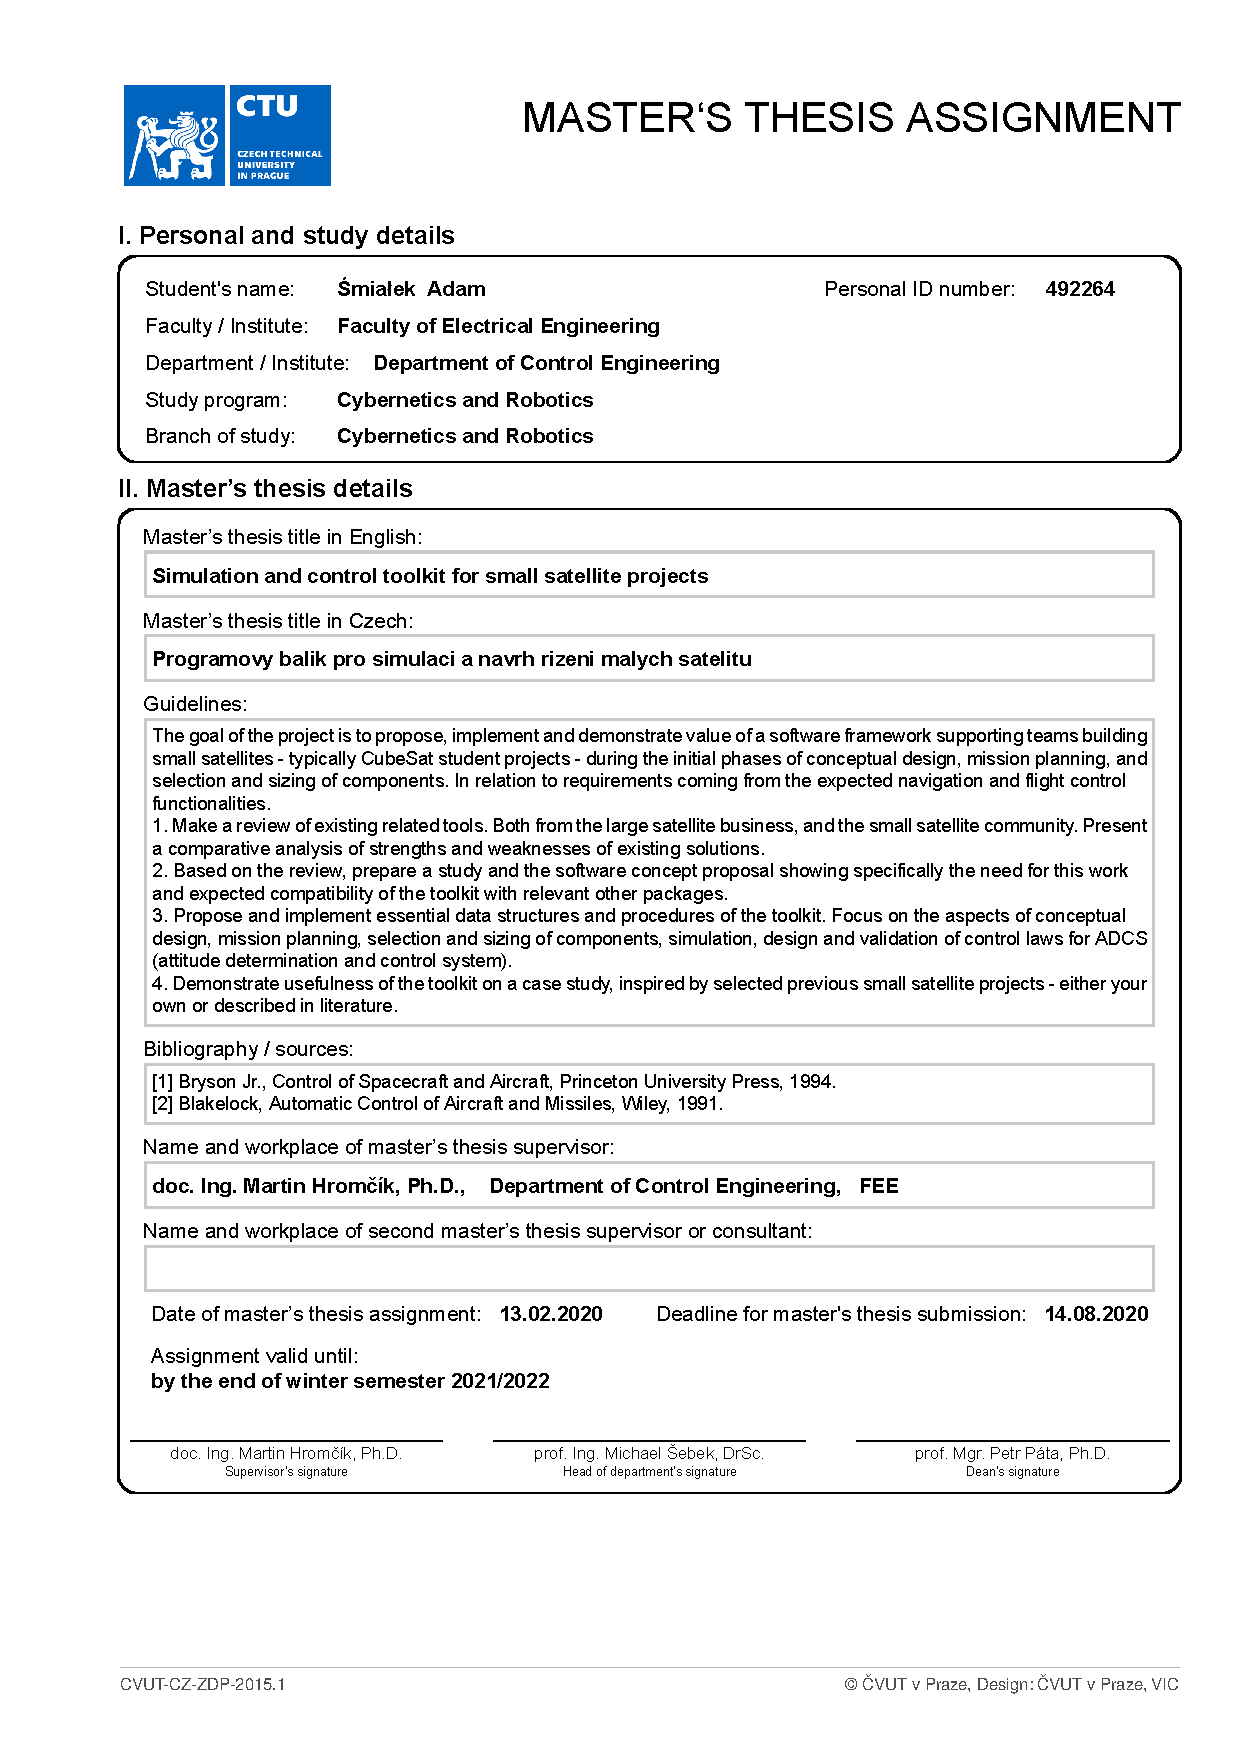
\includepdf[page={1,2}]{misc/Smialek_assignment.pdf}

% \newpage\null\thispagestyle{empty}\newpage
\clearpage
\hspace{0pt}
\vfill
\section*{Declaration}

% I hereby declare that the presented thesis is my own work and that I have cited all sources of information in accordance with the \textit{Guideline for adhering to ethical principles when elaborating an academic final thesis}.\\[0.1cm]

% I acknowledge that my thesis is subject to the rights and obligations stipulated by the Act No. 121/2000 Coll., the CopyrightAct, as amended. In accordance withArticle 46(6) of the Act, I hereby granta nonexclusive authorization (license) to utilize this thesis, including any and all computer programs incorporated therein or attached there to and all corresponding documentation (hereinafter collectively referred to as the "Work"), to any and all persons that wish to utilize the Work.\\[0.1cm]

% Such persons are entitled to use the Work for non-profit purposes only, in any way that does not detract from its value.\\[0.1cm]

% This authorization is not limited in terms of time, location and quantity.\\[1.0cm]

I declare that the presented work was developed independently and that I have listed all sources of information used within it in accordance with the methodical instructions for observing the ethical principles in the preparation of university theses.\\[1.0cm]

\dots\dots\dots\dots\dots\dots\dots  \hfill \dots\dots\dots\dots\dots\dots\dots \\
Place, date  \hfill Signature\\
\clearpage
\newpage\null\thispagestyle{empty}\newpage
\clearpage
\section*{Abstract}

% The process of effective spacecraft project management, from the conception of the idea, through production, to disposal, features high costs and often various unpredictable risks. Due to this, a project life cycle is usually divided into distinct phases, allowing for introduction of conducting product reviews within rigid time-frames.

Spacecraft project management calls for division of project lifetime into phases, with specific goals to be fulfilled at the end of each phase. During first few phases a \ac*{pdr} has to be conducted, after which top-level hardware design is not to be changed. This thesis describes a process of creating and demonstrates a software framework supporting teams building small satellites - typically CubeSat student projects - during initial phases of conceptual design, mission planning, and selection and sizing of hardware components. The scope of the thesis covers review of available tools for satellite mission and control system design, then it proposes a self-made MATLAB/Simulink toolbox - Spacecraft Control Architecture Rapid Simulator (SCARS) Toolbox, as a open source tool with gentle learning curve and ease of reverse engineering approach. In further parts of the thesis examples of usage are provided, and conclusions and descriptions of problems are presented. In the end, this thesis should not only serve as a description of SCARS toolbox, but also as an insight into the task of building a small satellite simulation.
\clearpage
\newpage\null\thispagestyle{empty}\newpage
\clearpage
\hspace{0pt}
\vfill
\section*{Acknowledgement}
\clearpage
\newpage\null\thispagestyle{empty}\newpage
\begingroup
    % \setcounter{tocdepth}{2}
    \setlength{\parskip}{0cm}
    \tableofcontents
\endgroup
\clearpage


\renewcommand{\arraystretch}{1.08}
\printacronyms[name = {Abbreviations}, sort = true]
\clearpage

\renewcommand{\arraystretch}{1.2} %
\setlength{\parskip}{0.25cm}
\pagenumbering{arabic}
\setcounter{page}{14}

\nocite{*}
\section{Introduction}\label{sec:introduction}
    % \todo[inline]{Here goes short introduction with mention that this is a work about \acf{scars}}
    The idea to create a simulation and control toolkit for small satellite projects was a byproduct of work done on IRISC project by the author of this thesis. IRISC, or "InfraRed Imaging of astronomical targets with a Stabilized Camera", was a project realized as a part of \ac{bexus} programme. The goal of the IRISC experiment was to obtain images in the \ac{nir} spectrum from astronomical targets. Possible targets included the Andromeda Galaxy, Pinwheel Galaxy, Iris Nebula, Eagle Nebula and Starfish Cluster. The images were obtained using a highly stabilized telescope with NIR camera mounted on a \ac{bexus} balloon. Author's responsibility covered the design of the control subsystem of the experiment. The stabilization was achieved by a gimbal-like system, to obtain high quality images while being on a moving platform\cite{irisc-sed}. The design of the control system was based on already existing models. Nevertheless, students with lack of previous practical experience in that field regarded it as a complex task. This has proven to be especially challenging during early stages of experiment design.

    The process of effective space-related project management - from the conception of the idea, through production, to disposal - features high costs and often various unpredictable risks. Due to aforementioned problems, a project life cycle is usually divided into distinct phases, allowing introduction of conducting product reviews within rigid time-frames. An example of such workflow, adopted by most major agencies such as ESA\cite{managementecss} and NASA\cite{kapurch2010nasa}, is a division of the project life cycle into phases, as presented on \autoref{fig:phases}. While the design of a project is often an iterative process, the phases and reviews that conclude them exist as a checkpoints, after which the design of the project is to be unchanged, on a level of details progressing as phases do. For example, Phase B is usually ended by the \ac{pdr}. In the case of a spacecraft, for the \ac{pdr}, a major architecture parameters have to be defined, such as volume and weight ramifications, top-level designs of solutions for major requirements need to be presented - for a practical example: for high-resolution Earth observation mission the type of the actuators which fulfills precision requirements has to be chosen.

    \begin{figure}[H]
        \centering
        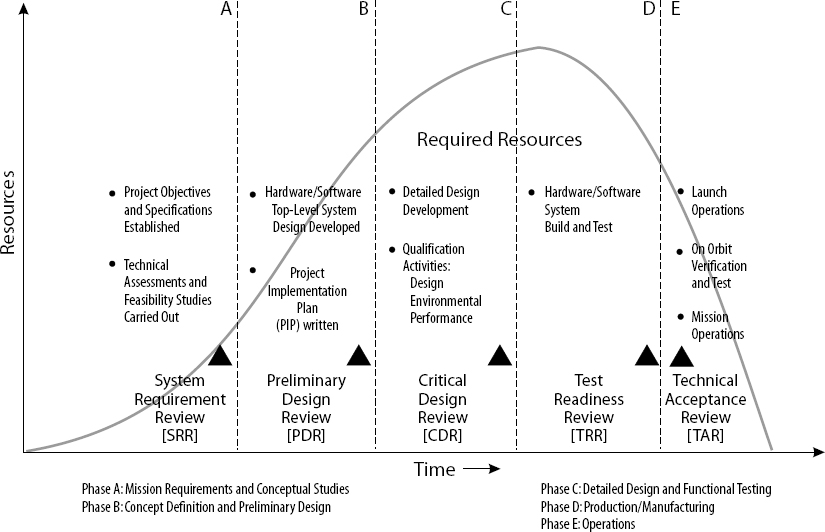
\includegraphics[width=1\textwidth]{1-introduction/phases}
        \caption{Typical space project phases and its life cycle\cite{nguyen2000effective}}
        \label{fig:phases}
    \end{figure}

    Taking the experience of how challenging and time-consuming was the process of learning how to produce a reliable simulation of IRISC control system and the knowledge of significance of preliminary design, author decided to produce and publish a simulation that is a useful for purposes of initial spacecraft design and for beginner engineers to learn how to build a reliable simulation. 
    
\subsection{Scope}
    The thesis covers the process of development of the toolbox for rapid prototyping of satellite's control systems. \autoref{sec:introduction} describes the aim of this work and discusses the topic of prototyping tools. \autoref{sec:toolbox} goes into details about the architecture, the features and methods of implementation of a toolbox created to fulfil the aims of the thesis - the \ac{scars} Toolbox. In addition it includes the description of methods of connecting \ac{scars} with various visualization tools. \autoref{sec:documentation} explains the documentation and usage of \ac{scars}, while in \autoref{sec:examples} there are examples of real life applications of the toolbox. Finally, \autoref{sec:conclusions} discusses the conclusions from the development process and the possibilities for improvements of \ac{scars}.

\subsection{Aim}\label{sec:aim}
    The aim of this thesis work is to build and provide a ready to use open source product - a toolbox for small and low budget satellite projects.  The toolbox features allow conducting initial design of spacecraft's \ac{adcs}, which means that is provides tools for, i.a. simulation of spacecraft orbit, testing the feasibility of various actuation methods and testing the effectiveness of different control algorithms in given use cases. That software would then allow smaller and inexperienced teams of spacecraft designers to better prepare for design milestones like \ac{pdr}, when there is not enough time to create a full simulation of their spacecraft \ac{adcs} subsystems. Besides the toolbox being a tool for practical use, the thesis also serves as as a review of available solutions, so it can be used by future control engineers as a learning material. The idea is that some parts of the proposed model cab be removed from the model while the students, for learning purposes, are tasked with designing a substitution.

    For the purposes of later evaluation of how the solutions proposed in this thesis fulfil the goals stated in the preceding paragraph, a following list of objectives was compiled:

    \begin{itemize}
        \item \textbf{Conduct a review of existing tools for preliminary spacecraft design}, focusing on mission planning and \ac{aocs} subsystem;
        \item \textbf{Create a spacecraft dynamics and \ac{aocs} model}, to be used with minimal set-up;
        \item \textbf{Assemble a library of models}, to be used by other beginner control engineers;
        \item \textbf{Provide a documentation of the toolbox}, explaining not only the purpose and operating principles of individual parts, but the process of using the toolbox to conduct a preliminary design of spacecraft \ac{aocs} subsystem;
        \item \textbf{Share the toolbox to be available online}, with principles of open-source software in mind.
    \end{itemize}

    Furthermore, the objectives that are set for the design of the toolbox itself are described in Chapter \ref{toolbox:objectives}.

% \subsection{Digital prototyping tools}
% \todo[inline]{refer to CAE software}
    % \dots\textit{description of CAD software}\dots
    % Prototypes are created to validate a design  an idea for the solution of a problem or

\subsection{Already existing tools}\label{sec:review}
    % ... This is to show that, while the toolbox for \ac{adcs} prototyping or development is not an innovative idea, but since some existing solutions are not best fit for the job of rapid prototyping and others are unavailable or paid, there is a need for a new, open-source one.

    The idea for a toolbox for spacecraft mission design and \ac{aocs} simulation is not a novelty. Various solutions are available, ranging from very robust commercial software packages to open-source implementations of individual features for use as a part of MATLAB framework.

    The aim of this section is to prove that despite the fact that the solutions for spacecraft prototyping are available, the need for open-source, easy-to-sue and modify toolbox still remains. Below a list of selected software solutions that fit the most objectives stated in \autoref{sec:aim} is stated, with explanation on the details, their features and the features which they lack and that discussed toolbox should have.

    \subsubsection{MATLAB CubeSat Simulation Library}
        % \todo{how to write that it was considered to expand this rather than develop own toolbox}
        CubeSat Simulation Library is a part of Aerospace Blocks created by MathWorks Aerospace Products Team. This library provides tool for modeling motion and dynamics of CubeSats and nanosatellites. It provides the most basic features, e.g. the simulation of pre-set attitude scenarios, basic actuators and sensors models and integration with MATLAB's Virtual World visualization tools.
        
        \begin{figure}[H]
            \centering
            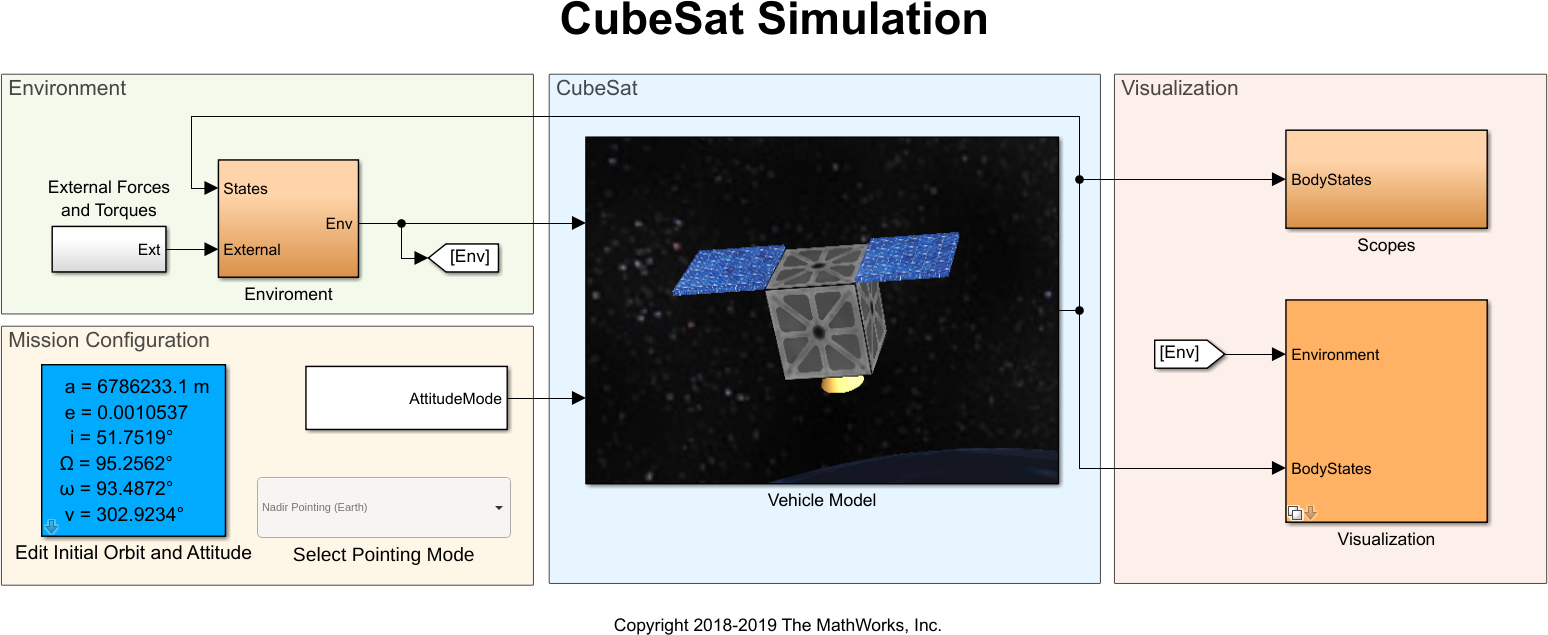
\includegraphics[width=1\textwidth]{1-introduction/matlab_cubesat}
            \caption{Top-level view of the example project of the MATLAB CubeSat Simulation Library}
            \label{fig:matlab_cubesat}
        \end{figure}

        This library, while conceptually most similar to the \ac{scars}, lacks some functionalities. For example, for actuators, it provides only general models for perfect and second-order actuators. In \ac{scars}, the actuators are full models, which allows not only reducing the number of layers of abstraction between the user and the simulation, but also for tasks like calculation of energy expended by the actuator. Moreover, this toolbox is sparsely documented - while most functionalities are described within their Simulink block masks, there is no comprehensive guide about how to use them in own models\cite{matlabcubesat}.

    \subsubsection{PrincetonSATELLITE Spacecraft Control Toolbox}
        \begin{figure}[H]
            \centering
            
\includegraphics[width=0.7\textwidth]{1-introduction/princeton.png}
            \caption{PrincetonSATELLITE Systems logo\cite{princetonlogo}}
            \label{fig:princeton}
        \end{figure}
        PrincetonSATELLITE Spacecraft Control Toolbox is a commercial solution for building spacecraft Simulations. It contains over two thousand functions for attitude and orbit dynamics, simulation, estimation, analysis and design. This is the most robust and comprehensive toolbox available, includes online API, accessible documentation and additional modules for unique applications like formation flying, fusion propulsion or solar sails. The toolbox is very robust, allowing the user to conduct long term simulations, but is also useful for short term simulations, like maneuver analysis and launch simulation. PrincetonSATELLITE Toolbox is a versatile and comprehensive tool and would be the best choice for most use-cases, yet it is a paid solution and even the cheapest option - CubeSat Edition - may be out of price range for smaller teams\cite{princeton}.

    \subsubsection{PROPAT Toolbox}
        PROPAT is a small set of functions in Matlab to simulate and propagate orbit and attitude of an Earth's satellite, developed by the single person as an open-source toolbox. Several functions allow to transform between orbit and attitude coordinates and for propagation or rigid body attitude. PROPAT contains only MATLAB scripts, which while useful and can be used as a part of the simulation, do not combine into a model of a whole spacecraft's \ac{adcs} subsystem\cite{propat}.

    \subsubsection{GAST Toolbox}
        \begin{figure}[]
            \centering
            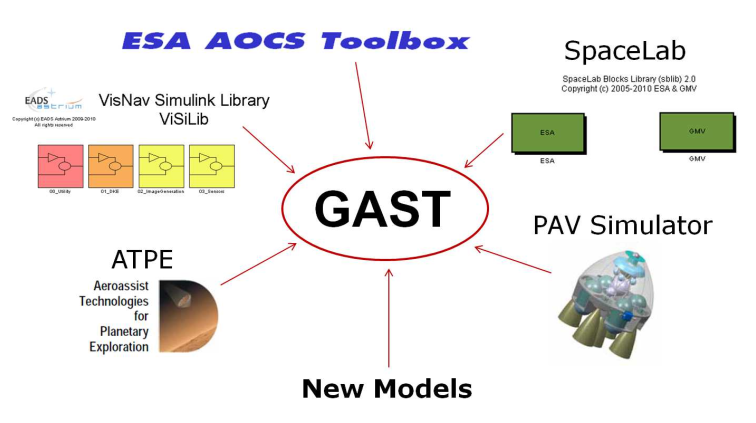
\includegraphics[width=1\textwidth]{1-introduction/gast}
            \caption{Representation of the consolidation of TEC-ECN toolboxes}
            \label{fig:gast}
        \end{figure}

        The GAST toolbox is the result of the consolidation of several toolboxes available in \ac{tec} of \ac{estec}, such as the \ac{aocs} Toolbox, the SpaceLAB library, the ViSiLib library, the ATPE simulator, and the PAV simulator. In addition to consolidating these toolboxes, new models were developed for the GAST toolbox according to the needs of the section. \autoref{fig:gast} shows a pictorial representation of the consolidation of the toolboxes of TEC-ECN. This software was developed in \ac{tec} in 2008, but since it is a product of \ac{esa}, it is not available for wider audience \cite{gast}.

    \vfill
    \subsubsection{User-created modules available on MathWorks MATLAB Central}
    MATLAB is one of the most popular scripting language between engineers, and along with Simulink package it provides tools helpful for simulating mechanical systems. Therefore, numerous modules and packages created by the users can be found online.
    
    MATLAB Central is a network for asking questions about MATLAB software, discussing solutions and sharing MATLAB and Simulink solutions and files\cite{matlabcentral}. On a subsection called File Exchange many files are available to use within MATLAB framework, some of them relevant to spacecraft design. The most notable examples are listed below.
    \clearpage

        \paragraph*{SAT-LAB}\hspace{0pt}\\[0.1cm]
            % \todo[inline]{https://www.mathworks.com/matlabcentral/fileexchange/63344-sat-lab-a-matlab-graphical-user-interface-for-simulating-and-visualizing-keplerian-satellite-orbits}
            SAT-LAB is a MATLAB-based Graphical User Interface (GUI), developed for simulating and visualizing satellite orbits. The primary purpose of SAT-LAB is to provide a software with a user-friendly interface that can be used for both academic and scientific purposes. While a useful tool, it is only suitable for initial mission planning\cite{satlab}.

        \paragraph*{Satellite Orbit Modeling}\hspace{0pt}\\[0.1cm]
            % \todo[inline]{https://www.mathworks.com/matlabcentral/fileexchange/54877-satellite-orbit-modeling}
            A collection of MATLAB scripts used for modelling of satellite's perturbed motion with special perturbations approach. Despite being very robust, as it can be applied to any problem in celestial mechanics, this module is useful for orbit modeling, not \ac{aocs} system design \cite{som-matlab}.
            
        \paragraph*{Smart Nanosatellite Attitude Propagator (SNAP)}\hspace{0pt}\\[0.1cm]
            % todo[inline]{https://www.mathworks.com/matlabcentral/fileexchange/68652-smart-nanosatellite-attitude-propagator-snap}
            The Smart Nanosatellite Attitude Propagator is an attitude propagator for satellites that can be used to analyze the environmental torques affecting a satellite and to design and analyze passive attitude stabilization techniques, such as Passive Magnetic Stabilization, Gravity Gradient Stabilization and Aerodynamic stabilization. This model is the most relevant one for the scope of this thesis, but it lacks possibility to model active attitude stabilization techniques \cite{snap}.

        \paragraph*{Satellite Orbits: Models, Methods and Applications}\hspace{0pt}\\[0.1cm]
            % \todo[inline]{https://www.mathworks.com/matlabcentral/fileexchange/54840-satellite-orbits-models-methods-and-applications}
            Rather than spacecraft or orbit model, it is a collection of exercises for book \textit{Satellite Orbits: Models, Methods and Applications}. As educational means, the exercises are interesting an refer at least partially to the problem of control system design - mainly GPS sensor. Yet this is not a toolbox by any means \cite{orbitsaddon}.
        
        \paragraph*{Apollo 11 Moon Landing - 50th Anniversary Model}\hspace{0pt}\\[0.1cm]
            % https://www.mathworks.com/matlabcentral/fileexchange/72127-apollo-11-moon-landing-50th-anniversary-model
            This example shows how the engineers who worked on the Apollo Lunar Module digital autopilot design could have used Simulink, Stateflow, Aerospace Blockset and Simulink 3D Animation if they had been available in 1961. Although it is a very notable example of how MATLAB software family can be used to simulate a whole mission, to use it for either own spacecraft or educational purposes would require much more reverse engineering and modifications than creating a new model \cite{apollo}. 

    \subsubsection{Overview}
        To summarize, software which helps spacecraft control engineers definitely is available. Yet, there is no solution which would have all the requirements that the product of this thesis tries to fulfil. The list of features that could be expected from a tool discussed in \autoref{sec:aim} is presented in \autoref{table:features}, with comparison of their inclusion in the examined software.

        \begin{table}[H]
            \adjustbox{max width=\textwidth}{{\renewcommand{\arraystretch}{1.6}
                        \centering
                        \begin{tabular}{C{2.5cm} | C{3cm} C{3cm} C{3cm} C{3cm} C{3cm} }
                        
                            \textbf{Feature}            & \textbf{MATLAB CubeSat Simulation Library} & \textbf{PrincetonSATELLITE Spacecraft Control Toolbox} & \textbf{PROPAT Toolbox} & \textbf{GAST Toolbox}  & \textbf{Smart Nanosatellite Attitude Propagator (SNAP)}  \\
            \hline 
                            Orbit propagation           & Yes                               & Yes                                           & Yes            & Yes           & Yes                                             \\
                            Mission planing             & No                                & Yes                                           & Partial        & No            & No                                              \\
                            Actuators and sensors model & No                                & Yes                                           & No             & Yes           & Only permanent magnets                          \\
                            Sensor fusion               & No                                & Yes                                           & No             & Yes           & No                                              \\
                            Control algorithms          & Partially                          & Yes                                           & No             & Yes           & No                                              \\
                            Environment simulation      & No                                & Partial                                       & No             & Yes           & Yes                                             \\
                            Parts database              & No                                & No                                            & No             & Yes           & No                                              \\
                            Availability                & {\small With MATLAB Aerospace Blockset}    & Fully commercial                              & Free online    & Not available & MATLAB File                                     \\
                            Documentation available     & Partial                           & Yes                                           & Yes            & Partial       & No                                              \\
                            Open source                 & Partially                         & No                                            & Yes            & No            & {\small Yes, apart from MATLAB back end}                 \\
                            %\hline just no
                        \end{tabular}}}
                        \caption{Comparison of features included in various software}\label{table:features}
                    \end{table}

\section{Spacecraft Control Architecture Rapid Simulator (SCARS) Toolbox}\label{sec:toolbox}
    To fullfil the main objective of this thesis, that is to provide a satellite control system prototyping toolbox the community of beginner control engineers, a self-made solution is proposed. This chapter provides the insight into the architecture of \ac*{scars} Toolbox, a software framework created in MATLAB and Simulink. First the main objectives of that solution are stated, then architecture of \ac{scars} is described, to give the initial description of how the toolbox can be used. In following sections the principles of operation of each major part of the toolbox, and how they were implemented, are presented.

    The inputs of \ac{scars} Toolbox - whether used as a parts library and integrated into own project, or as ready-made modular simulation - are parameters of spacecraft hardware, such as for example size of the satellite, trusters operational range, and initial mission parameters, for example time, Keplerian elements or initial body rates. The outputs of the toolbox are performances of each part and simulated behavior of the whole spacecraft, allowing the user to easily test different designs for their satellites.

    % This chapter describes the top-level architecture of the
    % \textit{Short description of the chapter.}
    % \textit{What SCARS means and what it is.}
    % \textit{Describe briefly what is the input and the output of the whole toolbox.}

\subsection{Objectives}\label{toolbox:objectives}
    The toolbox itself covers first two objectives of the the thesis. Following listing further specifies what should be expected of the end product and what features the users should be able to find in \ac{scars} Toolbox: 
    \begin{itemize}
        \item A model of orbital dynamics of Earth orbiting satellite;
        \item Models of most common satellite actuators and sensors and parametrize them so that actual hardware can be reproduced in simulation using values from datasheets;
        \item Modelled sources of environmental forces and torques, modeling most influential sources;
        \item Several most basic control methods;
        \item Simulink Custom Library, with all models masked for quick set up;
        \item Methods of conducting preliminary review of feasibility of used hardware components and control methods;
        \item Interfaces allowing the user to connect the toolbox with visualization software.
    \end{itemize}

\subsection{Choice of software}
    To fit with the objectives of accessibility and ease of modification MATLAB family of software was chosen. MATLAB is one of the most popular scripting language and with the addition of Simulink software it can become powerful tool with the ability to set up numerical simulations in short time. MATLAB is taught in most technical universities and there is significant number of both courses available online and materials for self-teaching. For one purpose (described in Section \ref{sec:ksp}) a Python script acting as a dataflow bridge was used, as it was a simplest method to solve a problem described in that chapter. Several other software solutions were used for visualization purposes, with the reasoning described in \autoref{sec:visualization}.

    Versatility of MATLAB may be attributed to the number of Add-Ons available for it. \ac{scars} Toolbox uses and requires the following modules:
    \begin{itemize}
        \item Aerospace Toolbox
        \item Navigation Toolbox
        \item CubeSat Simulation Library
    \end{itemize}
    
    %todo: cite courses and tutorials

\subsection{Architecture}
    \ac{scars} is divided into two parts: 1) Parts Library and 2) Modular Simulation. The Parts Library contains Simulink subsystems, which can be connected to form simulations of various complexity and for multiple scenarios. The other is a Modular Simulation, which can be set up with either MATLAB command line scripts or graphical user interface.

    \subsubsection{Parts Library}
        %TODO: Should I write something about the aim of the library?
        \ac{scars} Parts Library is a ready to use Simulink Custom Library, that is a collection of blocks available to use in Simulink models. All blocks in library downloaded alongside \ac{scars} are parametrized, masked and described to ease the integration of library parts into user simulation. The library is divided into specific sections:
        \begin{itemize}
            \item Satellite Dynamics
            \item Reference Frames Transformations
            \item Environment
            \item Actuators
            \item Sensors
            \item Control Algorithms
            \item Visualization
            \item Analysis
            \item Example scenarios
            \end{itemize}

        \begin{figure}[H]
            \centering
            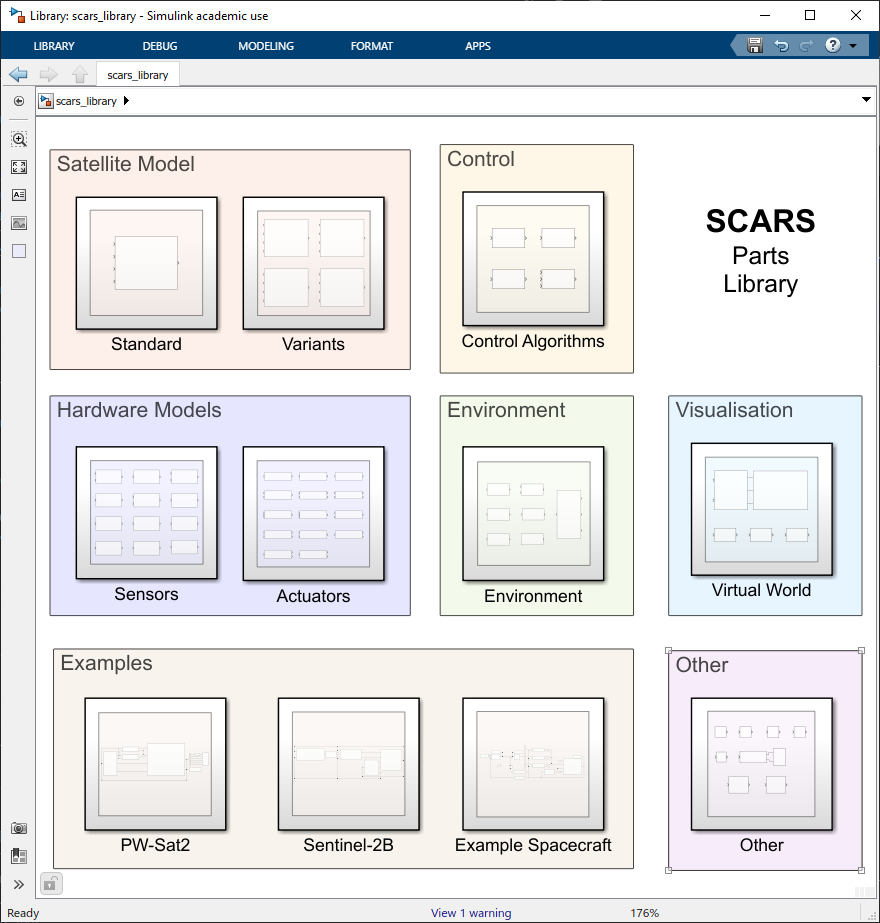
\includegraphics[width=1\textwidth]{2-toolbox/scars-library.png}
            \caption{SCARS Parts Library screenshot}
            \label{fig:scars-library}
        \end{figure}

    \subsubsection{Modular Simulation}
        \ac{scars} Modular Simulation is a ready-made simulink model available for setup using prepared scripts and \ac{scars} user interface. The model is a simulation of cube-shaped satellite, which can be set on specified orbit using various initialization methods, such as Keplerian elements in conjunction with Julian date time. (The initialization is further described in Chapter \ref{sec:documentation}). In the same manner, all actuators and sensors available in \ac{scars} library can be chosen. The Modular Simulation makes use of most available blocks, which can be commented out from the model, either by hand or using the user interface, to improve the speed of the simulation.

        \begin{figure}[H]
            \centering
            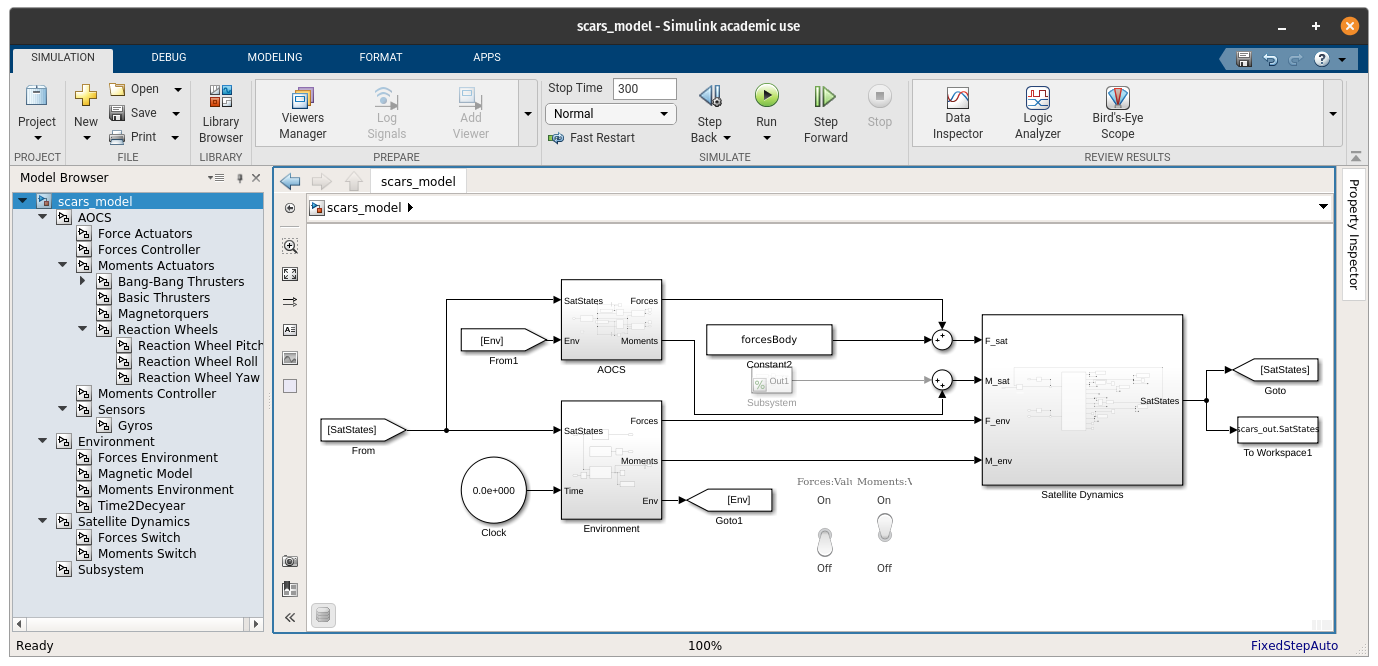
\includegraphics[width=1\textwidth]{2-toolbox/scars-model.png}
            \caption{SCARS Modular Simulation screenshot}
            \label{fig:scars-model}
        \end{figure}

\subsection{Orbit dynamics}

\subsection{Environment}
    Environment block is responsible for outputting few parameters, which are then used by the Satellite subsystem
    \begin{itemize}
        \item Gravity model
        \item Partial atmosphere?
        \item Sun's relative position and Earth's shadow
        \item Magnetic model
    \end{itemize}

    \subsubsection{Frames of Reference}
        Used: ECEF, NED

        Transformation from Keplerian Elemenets to Kartesian Coordinates

	% Note (vel eci to ecef): https://github.com/JuliaSpace/SatelliteToolbox.jl/issues/5

    Citation for orbital elements: \cite{vallado2001fundamentals}

    The body is assumed to be rigid?

    \subsubsection{Earths's Gravity Model}
        Simulink Aerospace Blockset \textbf{Spherical Harmonic Gravity Model}, EGM2008 Planet's Model

        Main centripetal force acting on a spacecraft on any orbit is 


        While equations ONE and TWO can be combined to faithfully model the influence of Earth's gravity field on the spacecraft, it was decided to 

        % Potentialy relevant: https://www.mathworks.com/matlabcentral/answers/349791-simulink-spacecraft-motion-integration-using-spherical-harmonic-gravity-model-problem

    \subsubsection{Partial Atmosphere}
        Earth's atmosphere is composed of complex layers that are loosely bounded basing on their composition and parameters. Man-made objects on Earth's orbit would be located in thermosphere, if their orbit is at least partially under $600km$ altitude above the surface of the Earth, or exosphere if above it. The former consists mostly of molecular hydrogen and nitrogen, while the latter also of hydrogen, helium ans carbon diaoxide. The main effects of the higher layers of atmosphere on the spacecrafts in \ac{leo} are drag, degradation of surface materials and spacecraft glow. For the toolbox, the only relevant effect is the first one, resulting in both aerodynamic force and aerodynamic torque acting on the spacecraft.

        Aerodynamic forces are created by spacecraft's movement through the atmosphere. The forces acting on the spacecraft are drag, lift and side slip force, but the only one taken into consideration will be the drag, acting on spacecraft's tangential velocity, since the other are of negligible magnitude. To calculate drag force, one has to use the following equation:
        \begin{equation}
            F_d = -\frac{1}{2}\rho C_d A v^2
        \end{equation}
        Where $C_d$ is the drag coefficient, $\rho$ is atmospheric mass density, $A$ is body area in a cross-section perpendicular to velocity vector and $v$ is the total velocity of the satellite with respect to the atmosphere. 

        \todo[inline]{Describe aerodynamic toruqe}

        \begin{figure}[hb]
            \centering
            \includegraphics[width=1\textwidth]{example-image-a}
            \caption{Model of Earth's atmosphere layers}
            \label{fig:atmosphere}
        \end{figure}

        The reference atmospheric model used in \ac{scars} is NRLMSISE-00, which takes date and position of the object in geographic coordinate system as inputs and outputs temperature and density of the atmosphere components. As it was built for satellite, it allows for altitudes up to $1000km$. In the toolbox, orbits above that are considered to have negligible impact of the atmosphere.

\clearpage
\subsection{Actuators}\label{sec:actuators}
    \begin{figure}[H]
        \centering
        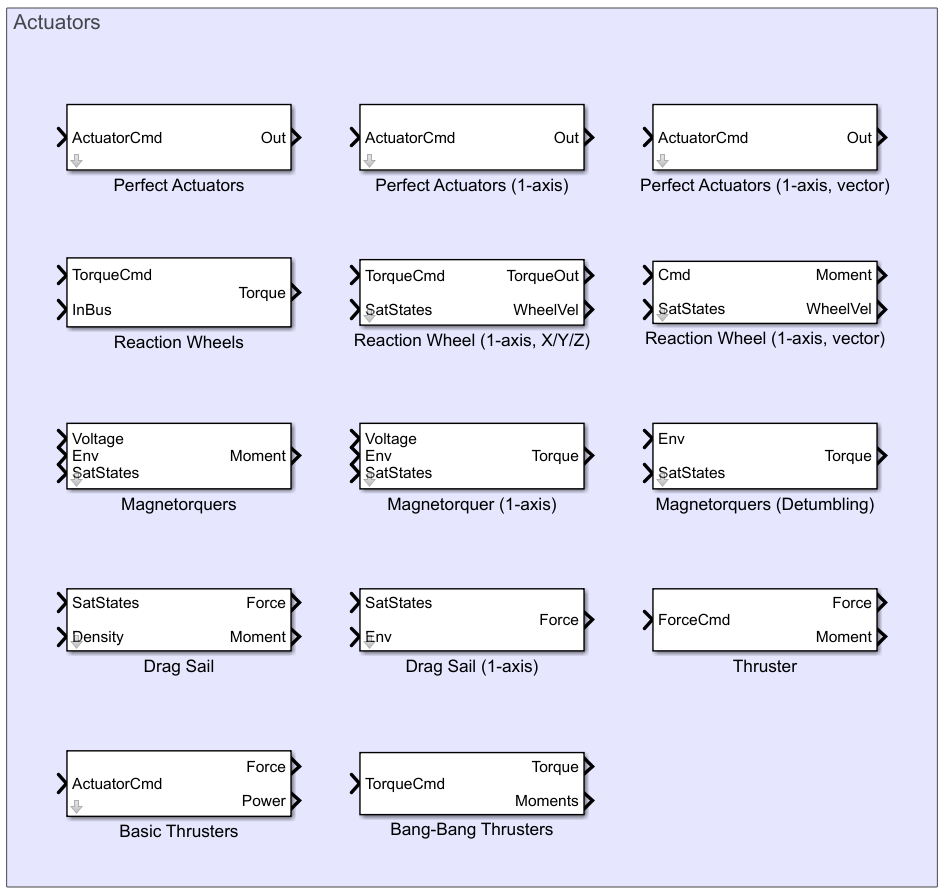
\includegraphics[width=0.7\textwidth]{2-toolbox/actuators.png}
        \caption{All Actuators blocks available in SCARS Parts Library}
        \label{fig:actuators}
    \end{figure}
    % \dots\textit{introduction}\dots
    In the following subsections, the descriptions of actuators included in \ac{scars} Toolbox are provided. All of them can be used in a model by themselves or in combination with any other number of actuators. The model linearization method described in \autoref{app:linearization} allows for using all provided actuators with all control methods described in \autoref{sec:control}. 

    \subsubsection{Ideal and Simple Actuators}
        Ideal Actuators are simply Simulink subsystems including unit gain. Their purpose is to serve as a placeholder, if other parts of ADCS subsystems are tested and simulation of actuator behavior is not necessary.

        Simple Actuators are ought to simulate most generic sources of errors in actuators, for the user to be able to create a more reliable placeholder for actuator not yet available in \ac{scars} Toolbox.


    \subsubsection{Thrusters}
        % https://www.cubesatshop.com/wp-content/uploads/2017/04/ENP-IFM-Nano-Thruster-Product-Overview.pdf
        % https://blog.satsearch.co/2019-07-10-cubesat-thrusters-an-overview-of-in-space-propulsion-products-for-small-satellites
        % \dots\textit(principle of operation)\dots

        \begin{figure}[H]
            \centering
            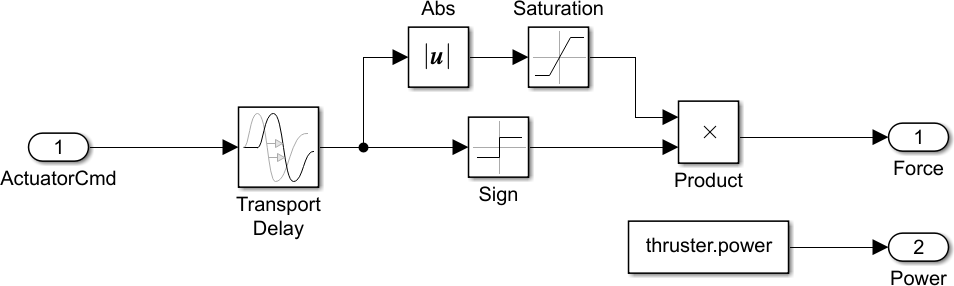
\includegraphics[width=0.8\textwidth]{2-toolbox/basic_thrusters.png}
            \caption{Directional Thruster model}
            \label{fig:basic_thrusters}
        \end{figure}

        One type of actuators that provide the source for external forces and torques acting on a spacecraft are gas thrusters. In case of small satellites, \ac{cgp} Systems are the most popular solution, since its simple design leads to smaller actuator mass and low power consumption. A \ac{cgp} system operates in a process of controlled ejection of compressed liquid or gas propellant. 
        
        Spacecraft thrusters can be used for orbit change maneuvers, rapid attitude changes, momentum dumping, nutation and adjusting spin rates. The main advantage of gas propulsion is that the thrust can be controlled with high precision and they can provide high forces and torques. Moreover, there is no need for desaturation of a thrusters, in opposition to reaction wheels. Nevertheless the requirement for propellant posses a problem for small satellites, making it a rare method of attitude control in CubeSats and other micro- and nanosatellites. 
        
        The key parameters, available for set up in \ac{scars} Toolbox Thruster model are: thrust range, nominal thrust, specific impulse, amount of propellant, total impulse, power consumption, mass and time delay to control. Same as in Simple Actuators, noise sources can be set up.

        In \ac{scars} Parts Library various versions of Thruster are available:
        \begin{itemize}
            \item \textbf{Directional Thrusters} - Effective forces are assumed to be located on spacecraft body axes, leading to the lack of external torques, hence this model can be used for orbit corrections and maneuvers.
            \item \textbf{Rotational Thrusters} - Effective forces are assumed to be axisymmetric, therefore there are no forces generated by the thrusters, so this configuration can be used for pure attitude control. Additional parameter required for this model is radial displacement for the thrusters. 
            \item \textbf{Bang-Bang Thrusters} - Thrusters that operate in bang-bang control mode, allowing for operation only with no or maximum thrust. Additional parameters required for this model are turn-on and turn-off thresholds in control signal. They can be used either in orbit or attitude control and in respective cases they follow the principles of Directional and Rotational Thrusters.
        \end{itemize}

        \begin{figure}[H]
            \centering
            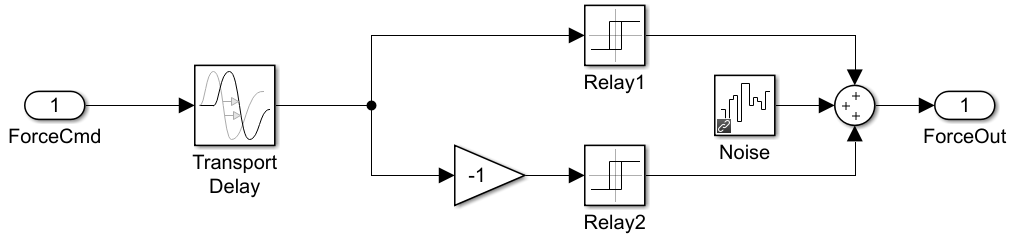
\includegraphics[width=0.8\textwidth]{2-toolbox/bang_bang.png}
            \caption{Bang-Bang Thruster model}
            \label{fig:bang_bang}
        \end{figure}


        For all thrusters models the only input is the control signal, while the outputs are fuel consumed and either generated force or torque. \ac{cgp} Systems also have a downside of decreasing thrust profile in relation with time, since thrust is correlated with the pressure of the propellant inside a tank. This property is not yet modeled in \ac{scars} Toolbox. %\dots\textit{should it be?}\dots

        % \begin{itemize}
        %     \item Thrust range;
        %     \item Nominal thrust \textit{(find a way to model change)}
        %     \item Specific impulse \textit{(and ranges)}
        %     \item Max propellant
        %     \item Total impulse
        %     \item Power consumption \textit{(at nominal thrust)}
        %     \item Mass
        %     \item Dimensions?
        %     \item Hot standby Power
        %     \item Time delay to control
        %     \item In both directions
        % \end{itemize}
        
        % \dots\textit{description of implementation}\dots

        % Bang-bang: https://apps.dtic.mil/dtic/tr/fulltext/u2/a291803.pdf
        % /resources/noise_description.pdf
        % \begin{figure}[H]
        %     \centering
        %     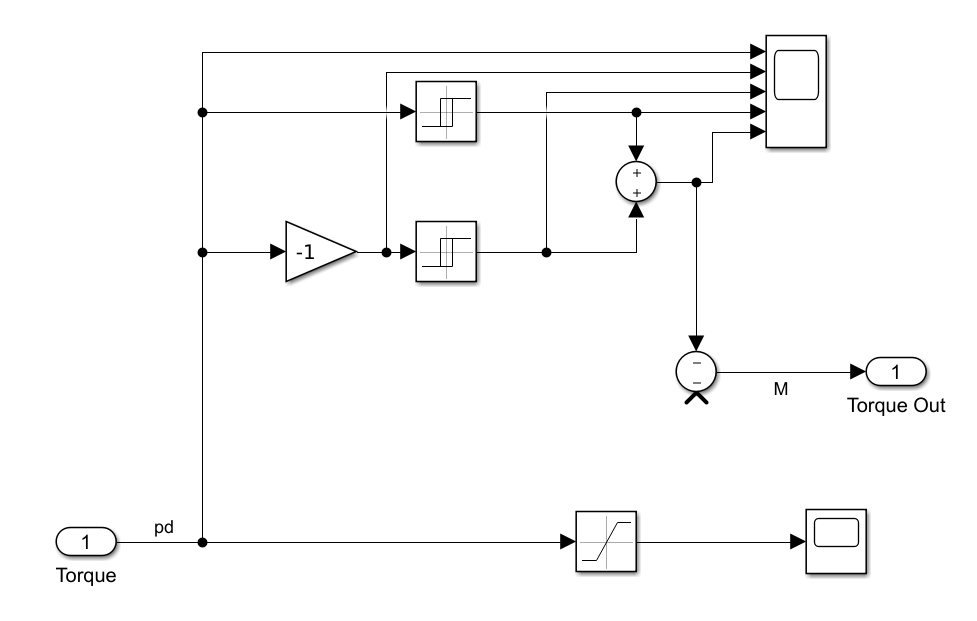
\includegraphics[width=1\textwidth]{2-toolbox/thru_simulink.png}
        %     \caption{Simulink Bang-Bang Thrusters model wrapper}
        %     \label{fig:bang_bang_simulink}
        % \end{figure}

    \subsubsection{Reaction Wheels}
        \begin{figure}[H]
            \centering
            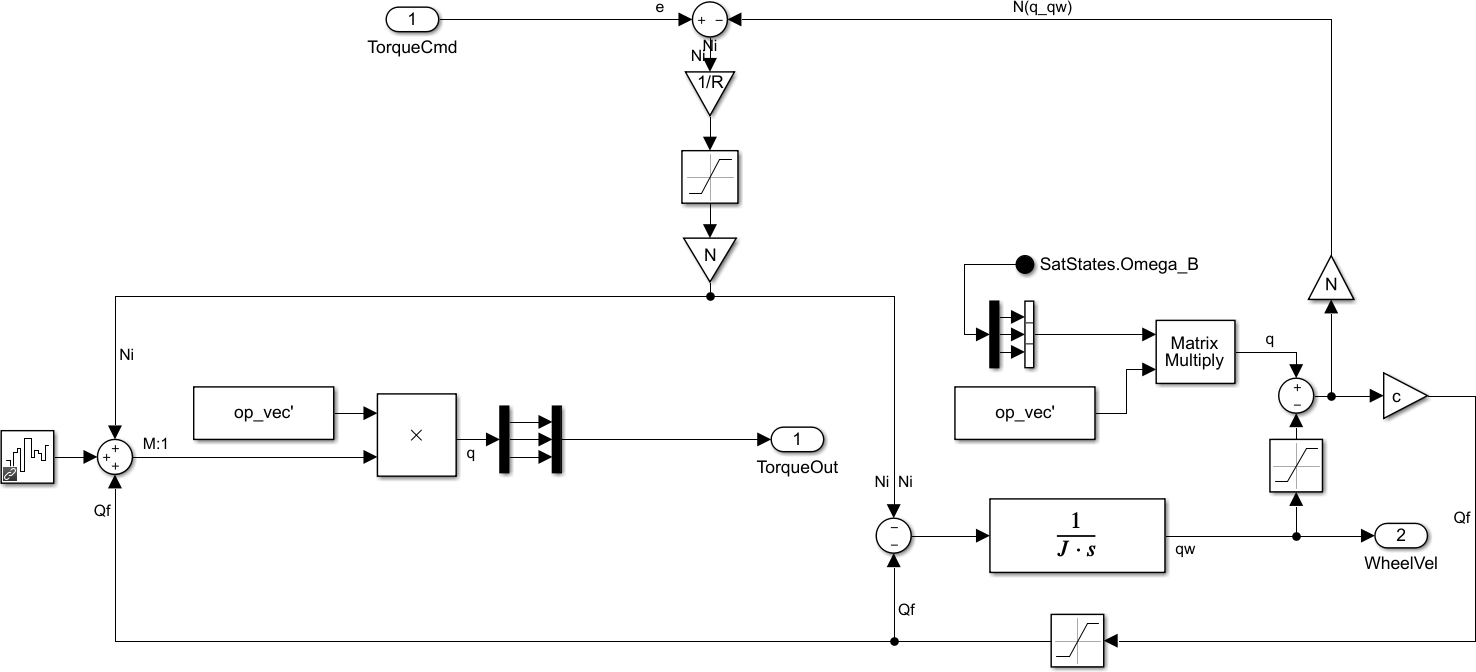
\includegraphics[width=1\textwidth]{2-toolbox/reaction_wheels.png}
            \caption{SCARS Reaction Wheel model}
            \label{fig:reaction_wheels}
        \end{figure}

        % Ideal to real: Bearing Noise, Transport Delay, Saturation, Quantization.
        
        Fast attitude control can be also achieved by the use of reaction wheels - mechanisms consisting of rotating flywheel and proportional electromagnetic torquer, such as DC motor. This allows very precise attitude maneuvers, with the possibility to eliminate most disturbance torques. Reaction wheels operate at around non-zero reference speed and change in their angular velocity imposes corresponding torque on the spacecraft. The disadvantage of this solution is that reaction wheels have fixed operating range and to achieve higher angular velocities for the spacecraft, the wheels have to be desaturated using another actuators. In CubeSats, for example, most commonly this would be solved by the addition of magnetorquers.

        In fast attitude control the motion around each spacecraft body axis can be considered to be decoupled from motion around two other axes. The equations of motion that describe the influence of reaction wheels angular velocity $\dot{q_w}$ on total angular momentum $H$ are as follows:
        
        % \begin{equation}
        \begin{align}
            I_y\dot{q} &= Ni+Q_f+Qdy\\
            \dot{\Theta} &= q\\
            J\dot{q_w} &= -Ni-Q_f\\
            Ri &= e - N(q-q_w)\\
            Q_f &= -c(q-q_w)\\
            H &= I_yq + Jq_w
        \end{align}
        % \end{equation}

        Where $e$, $i$, $R$ are respectively steering voltage, current in DC motor and armature resistance. $N$ is torque per unit current and $c$ is viscous friction coefficient. $Q_f$ is wheel bearing friction torque and $Q_{dy}$ stands for external disturbance torque. Said equations were modelled in the toolbox as it can be seen on \autoref{fig:reaction_wheels}. 

        The problem with modeling off-the-shelf reaction wheels is that datasheets rarely provide the value of viscous friction coefficient $c$ in the DC motor, therefore in \ac{scars} it is considered to be an optional parameter. 
        
        % Therefore to model this kind of actuator, \ac{scars} requires the user to only input following data, with $c$ being optional:
        
        % sources: bryson and this funny magnetorquer stuuff
        
        % \subsubsection{Gimbaled Momentum Wheel}

        %here goes the table


    \subsubsection{Magnetorquers}\label{sec:magnetorquer}
        % sources - "magnetorquer and nice stuff" pdf and sidi maybe?

        \begin{figure}[H]
            \centering
            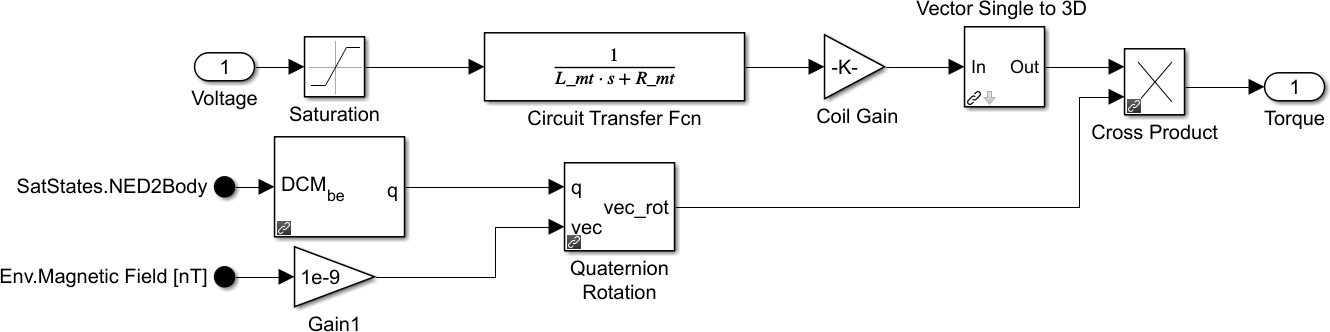
\includegraphics[width=1\textwidth]{2-toolbox/magnetorquer.png}
            \caption{SCARS Magnetorquer model}
            \label{fig:magnetorquer}
        \end{figure}

        A magnetorquer is an attitude actuator which uses Earth's geomagnetic field to generate controlling torque. The active part in the magnetorquer is the solenoid, which generates the magnetic dipole moment proportional to the current conducted by the coil. This interaction is described with the following equation:

        \begin{align}
            \tau_B = M \times B
        \end{align}

        Where $\tau_B$ is mechanical torque acting on the spacecraft, $M$ the generated magnetic moment inside of it and $B$ is the magnetic field density. As the product of a skew-symmetric matrix and a vector it takes a form of:

        \begin{equation}
            \begin{bmatrix}
            \tau_{Bx}\\ 
            \tau_{By}\\ 
            \tau_{Bz}
            \end{bmatrix}
            \begin{bmatrix}
            0 & B_z & -B_y\\ 
            -B_z & 0 & B_x\\ 
            B_y & -B_x & 0
            \end{bmatrix}
            \begin{bmatrix}
            M_x\\
            M_y\\
            M_z
            \end{bmatrix}                
        \end{equation} % cite SIDI heres

        \ac{scars} Magnetorquer block models a torque rod, a solenoid with a magnetic core. The magnetic moment of a rod magnetorquer is a function of rod current and parameters of the coil, as described in following equation:

        \begin{equation}
            M = I_M\frac{\pi lw}{4d}\left[\left( \frac{\left[ \left( \frac{l}{w} \right) -1\right]^{3/2}}{\left( \frac{l}{w} \right)\cosh^{-1}\left( \frac{l}{w} \right)-\left[\left( \frac{l}{w} \right)^2 -1\right]^{1/2}} \right)- 1 \right]
        \end{equation}

        Where $l$ is the length of magnetic core, $w$ is the width of it and $d$ is the diameter of the wire. $I_M$ is the current flowing through the rod, which can be described with a transfer function, where $L$ is the solenoid's inductance and $R$ its resistance:

        \begin{equation}
            I_M = \frac{V_M}{Ls+R}
        \end{equation}

        % interesting problem with B matrix being singular, SIDI page 186 (204 in pdf)

        % cite: GOOD MAGNE CITE - 10.1.1.565.8909.pdf

        The drawback of using magnetorquers for attitude control is that they are unfit for fast maneuvers. Moreover, since Earth's magnetic field density is inversely proportional to cube of distance from Earth's center, then without high grade sensors or on-board models, they do not allow precise maneuvering on higher orbits.


    \subsubsection{Drag Sail}
        \begin{figure}[H]
            \centering
            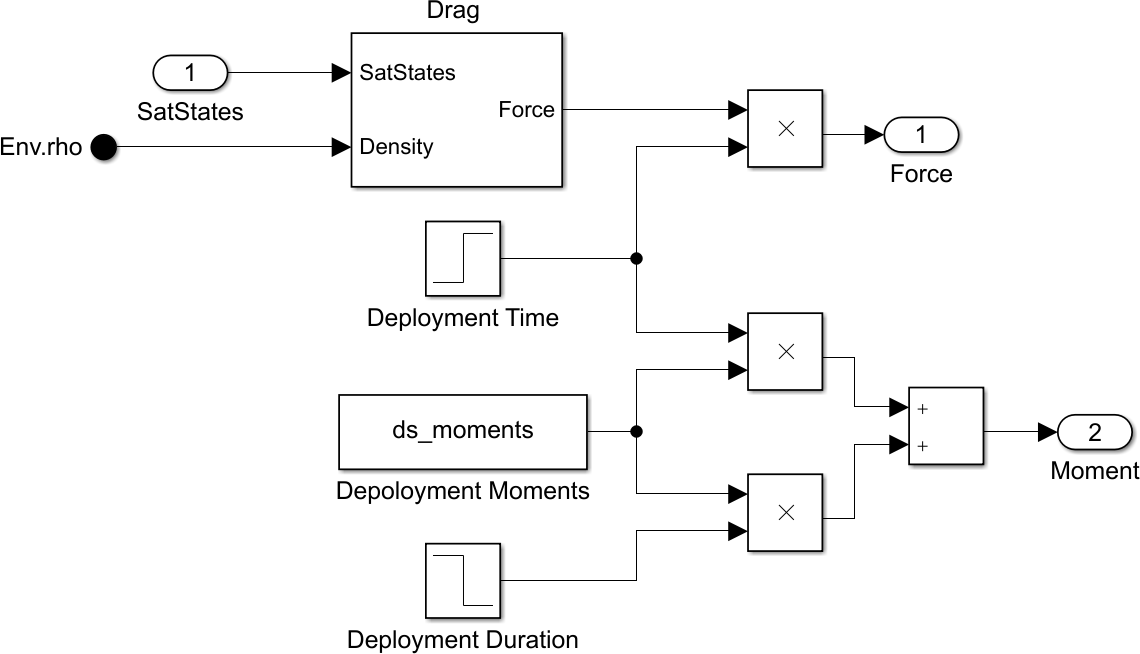
\includegraphics[width=0.8\textwidth]{2-toolbox/drag_sail.png}
            \caption{SCARS Drag Sail model}
            \label{fig:drag_sail}
        \end{figure}

        Drag sails use the occurrence of partial atmosphere (described in \ref{toolbox:atmosphere}) to lower satellite's tangential velocity and therefore to quicken the deorbitation of the spacecraft. The premise is to increase area-to-mass-ratio by deploying a large and lightweight structure near the planned end-of-life of the spacecraft. Due to this operating principle, drag sails are only relevant for low and medium mass spacecrafts and are applicable exclusively on \ac{leo}. To calculate the perturbing acceleration following equation is used:
        \begin{equation}
            F = -\frac{1}{2}\rho C_d A v^2sin\alpha
        \end{equation}
        Where $alpha$ is the angle between the sail's plane and satellite's velocity vector. Currently the moment of sail's deployment is not simulated in \ac{scars} toolbox.


\subsection{Sensors}
    For precise orbit, or attitude, determination both sensors and mathematical models have to be used. Spacecraft sensors can be divided into two types, based on the nature of the performed measurement. One type, inertial sensors reflect the rate of change, therefore any other source of measurement is needed, for initial value acquisition and integration error correction. On the other side there are reference sensors, providing absolute measurements. Sensors of this type measure external parameters, such as Sun's position or Earth's magnetic field intensity, which when compared against mathematical or empirical models can bare the information about satellite's position or attitude. This division is visible in \ac{scars} models, as inertial sensors require input of satellite states, while reference sensors need input from environment model.

    It is important to mention, that it is possible to model sensors with various degrees of fidelity and different focus. For example, the influence of mechanical parameters on output signal of gyroscope is significant, resulting in a need for modeling it with transfer function describing it's properties. On the other hand, in sensors such as star tracker the output is mostly processed in the software, therefore the focus is put on modeling the influence of spacecraft kinematics on the sensor, such as blinding the camera by the sun.

    \subsubsection{Ideal and Simple Sensor}
        Ideal Sensor is a Simulink subsystem block with unit gain inside, used for testing satellite behavior when sensor errors are not necessary to be taken into consideration.

        Simple Sensor is not modelling any specific type of sensor. It can take most parameters used to transform generic ideal sensor into model which corresponds to real hardware, that is: sampling frequency, measurement range and most common sources of errors.

        % In the toolbox the following sources of gyroscope errors are modeled:
        % \begin{itemize}
        %     \item Bias offset:
        %     \item Scale factor: 
        %     \item \ac{arw}: A high frequency noise term that has a correlation time much shorter than the sample time. Can be defined as white noise component on the sensor output. Specified either in $\frac{deg}{\sqrt{h}}$ or, as a power spectral density, in $\frac{(deg/h)^2}{Hz}$. % cite this here: http://citeseerx.ist.psu.edu/viewdoc/download?doi=10.1.1.210.1133&rep=rep1&type=pdf
        %     \item Quantization Error: An error which is caused by the digital quantization of output signal, obtained when sampling analog input.
        %     \item ...
        % \end{itemize}

        \dots\textit{description of implementation}\dots

    \subsubsection{GPS Receivers}
        The \ac{gps} is a \ac{gnss} owned adn operated by United States government. It allows for determining position, velocity and time using data taken from at least four \ac{gps} satellites.

        Previously using \ac{gps} receivers in \ac{leo} was burdened with technical challenges, as off-the-shelf components were mostly designed for terrestrial operations, not encompassing for example for large variations in the received signal Doppler frequencies. Recently smaller \ac{gps} receivers became available, even for CubeSat use, such as \textit{Venus838FLPx GPS Receiver}\cite{gpsdatasheet}, allowing for real time orbit determination using \ac{gps} navigation in smaller satellite projects.\cite{gomes2007real} When choosing a \ac{gps} receiver one must take several parameters into consideration: update rate, horizontal position accuracy, vertical position accuracy, velocity accuracy and failure rate.
        
        % \begin{itemize}
        %     \item Update rate
        %     \item Horizontal position accuracy
        %     \item Vertical position accuracy
        %     \item Velocity accuracy
        %     % \item Decay factor?
        %     \item Failure rate
        % \end{itemize}

        All listed parameters are set up in \ac{scars} \textit{GPS Receiver} part, but rather than designing a model from scratch, MATLAB's Navigation Toolbox function, \verb|gpsSensor()|, was nested inside a masked Simulink block. User can set all beforementioned parameters by editing \ac{gps} model's mask fields. Inputs of the model are satellite's true position and true velocity, and the outputs are position and velocity as computed by \ac{gps} receiver.


    \subsubsection{Accelerometers}
        \begin{figure}[H]
            \centering
            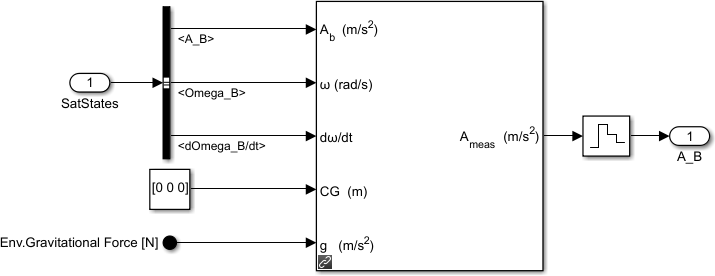
\includegraphics[width=1\textwidth]{2-toolbox/accelerometer.png}
            \caption{SCARS Accelerometer model}
            \label{fig:accelerometer}
        \end{figure}
        % accelerometer misalignment
        Accelerometers are force sensors, most often paired with gyroscopes as a part of \ac{imu} board. To measure acceleration three sensors are located with their axes mutually orthogonal and the force external to the board is measured (with the exception of the gravitational force, as it likewise influences the proof mass of the sensor). These measurements are integrated once to obtain the velocity of the spacecraft with respect to the inertial space, or twice to calculate estimated position.

        Accelerometer model in \ac{scars} is based on Three-axis Accelerometer from MATLAB Aerospace Blockset. It is masked to be easily integrated with any model produced with \ac{scars} Toolbox.

        % write something about second order dynamics

        % \dots\textit{description of implementation}\dots

    \subsubsection{Magnetometers}
        \begin{figure}[H]
            \centering
            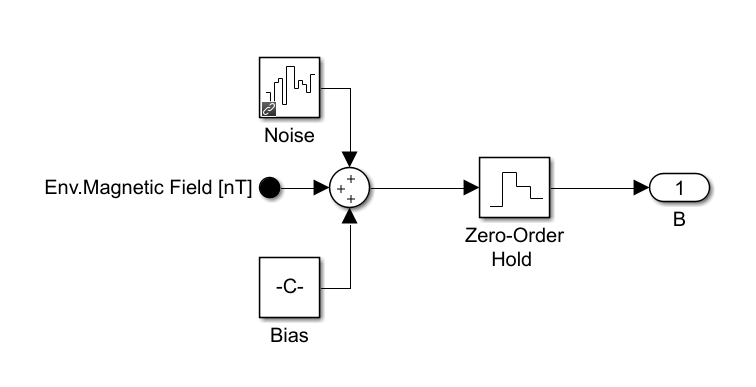
\includegraphics[width=1\textwidth]{2-toolbox/magnetometer.png}
            \caption{SCARS Magnetometer model}
            \label{fig:magnetometer}
        \end{figure}

        Making use of implemented Magnetic Field Model, a model of a set of magnetometers is available as a part of \ac{scars} Toolbox. From magnetometer sensors the measurements of direction and magnitude of magnetic field can be acquired. After comparison with Earth's magnetic model spacecraft's on board software conducts transformation from measured vector to one of the reference frames used by \ac{adcs} subsystem, providing information about its attitude. Magnetometers are reliable choice of sensors, as they are lightweight, consume low amounts of power, operate in wide temperature ranges. 
        %cite: MAGNETOMETERS - richard2008 (maybe)

        \dots\textit{description of implementation}\dots

    \subsubsection{Gyroscopes}
        % https://www.youtube.com/watch?v=anMzEbbbrp8
        % Parameters:
        % \begin{itemize}
        %     \item change over temperature
        %     \item zero rate level change over temperature [dps/*C] (but this can biased to get rid of the error, so is not necessary to model)
        %     \item sensitivity
        %     \item Measurement range
        %     \item Angle Random Walk (same Parameter as FFT and Power Spectral Density)
        % \end{itemize}

        \begin{figure}[H]
            \centering
            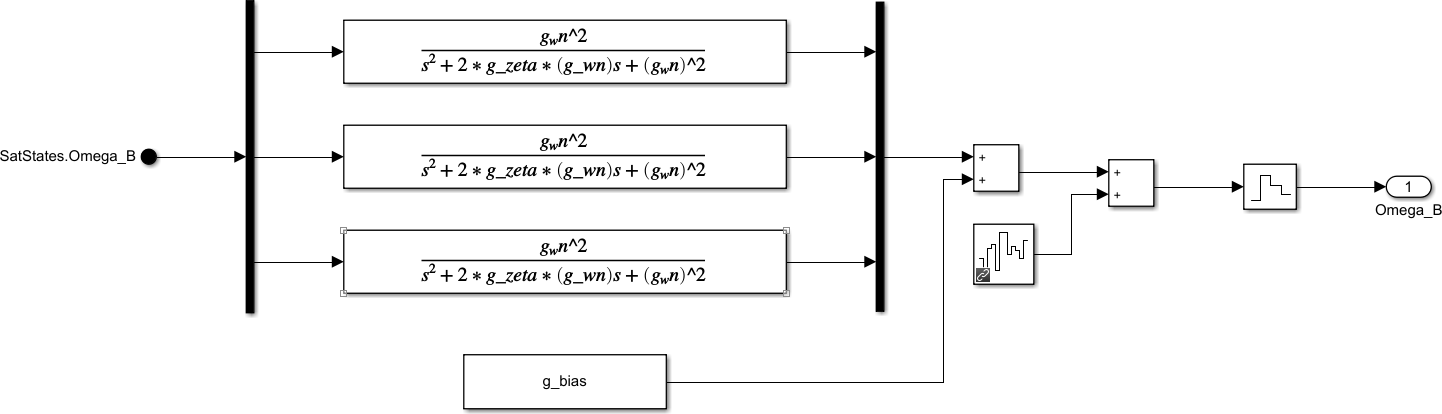
\includegraphics[width=1\textwidth]{2-toolbox/gyroscope.png}
            \caption{SCARS Gyroscope model}
            \label{fig:gryo_simulink}
        \end{figure}

        Gyroscopes, which fall under category of inertial sensors, measure angular rate around fixed axis. In smaller spacecraft, which is in great deal of \ac{scars} toolbox use-cases, the conventional spinning mass gyroscopes are rarely used, due to limitations in mass and size. Recent developments allow for use of much smaller and cheaper \ac{mems} gyroscopes, which are vibrating angular rate sensors. They were chosen to model for the toolbox, as of popularity in projects with highly restricted budget. \cite{armenise2010advances} Inside of vibrating gyroscope the Coriolis effect is a cause the vibrating core to produce a force acting on its support. The measurement of the force is used to determine the rate of rotation of the body around gyroscope axis. \ac{mems} gyros are similar to integrated circuits, which use the miniaturized version of mechanisms based on principles of operation of either vibrating wheels, tuning forks, resonant solids or similar common designs. \cite{bernstein2003overview} While, besides previously mentioned qualities, the upsides of \ac{mems} gyroscopes are availability of both analog and digital outputs, low power consumption and commercial availability. On the other hand, \ac{mems} gyros have shorter lifetime and lower performance when compare to pricier alternatives.

        % In the toolbox the following sources of gyroscope errors are modeled:
        % \begin{itemize}
        %     \item Bias offset:
        %     \item Scale factor: 
        %     \item \ac{arw}: A high frequency noise term that has a correlation time much shorter than the sample time. Can be defined as white noise component on the sensor output. Specified either in $\frac{deg}{\sqrt{h}}$ or, as a power spectral density, in $\frac{(deg/h)^2}{Hz}$. % cite this here: http://citeseerx.ist.psu.edu/viewdoc/download?doi=10.1.1.210.1133&rep=rep1&type=pdf
        %     \item Quantization Error: An error which is caused by the digital quantization of output signal, obtained when sampling analog input.
        %     \item ...
        % \end{itemize}
        
        % write something about second order dynamics

        In \ac{scars} the gyroscope model, as seen on \autoref{fig:gryo_simulink}, includes a second order transfer function, describing the system using parameters such as natural frequency, bandwidth, damping ratio, but also it includes gyroscopic bias and noise source, in attempt to transfer ideal gyroscope into real sensor. 

        % \dots\textit{work in progress}\dots

    %    - Cite this: \cite{kapeelmodeling} % for errors

    % \subsubsection{Inertial Measurement Units}

    \subsubsection{Star Tracker}
        % https://www.youtube.com/watch?v=anMzEbbbrp8
        % Parameters:
        % \begin{itemize}
        %     \item change over temperature
        %     \item zero rate level change over temperature [dps/*C] (but this can biased to get rid of the error, so is not necessary to model)
        %     \item sensitivity
        %     \item Measurement range
        %     \item Angle Random Walk (same Parameter as FFT and Power Spectral Density)
        % \end{itemize}

        \begin{figure}[H]
            \centering
            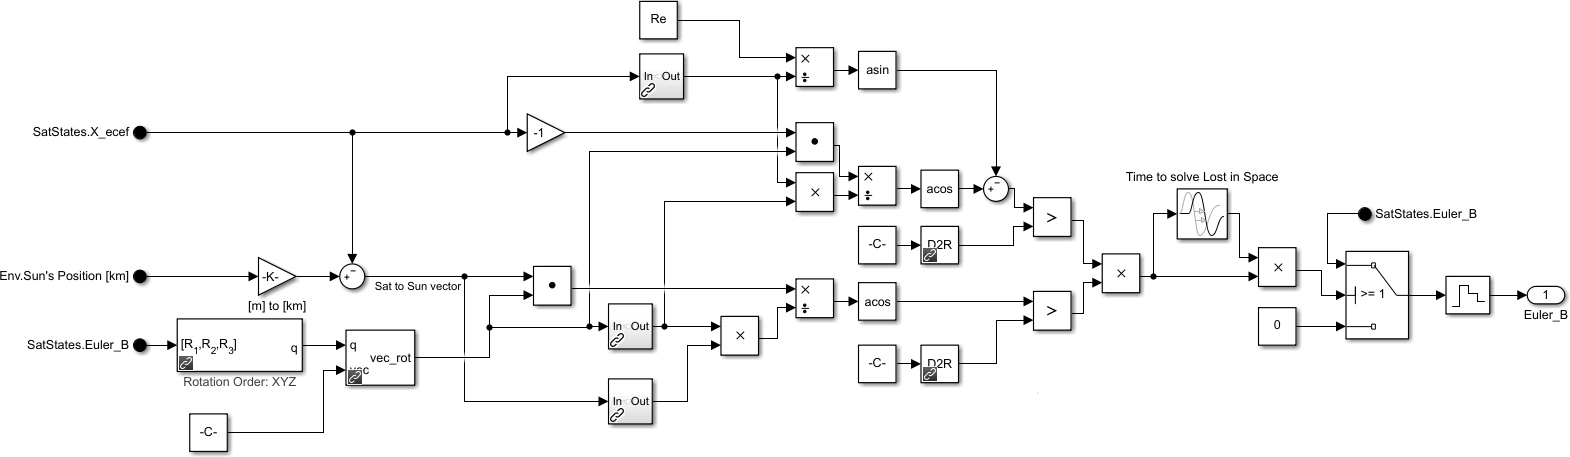
\includegraphics[width=1\textwidth]{2-toolbox/star_tracker.png}
            \caption{SCARS Star Tracker model}
            \label{fig:star_tracker}
        \end{figure}

        A star tracker is an complex attitude sensor, providing the most accurate determination within available commercial solutions. It consist of optical camera and wide array of processing algorithms, which allow to read the position of the stars from captured image and to compare that positions to database of known and visible stars to find the attitude of the spacecraft. Moreover, it can do so without a-priori knowledge, using lost-in-space algorithm\cite{delabie2016star}.

        As simulating stars position to achieve high fidelity star tracker model and using parameters such as camera resolution and algorithm accuracy and precision, it was decided to assume ideal output from star tracker and to focus on mechanical problems, such as blinding the sensitive camera sensor by light from the Sun or reflected by the Earth. As it can be seen on \autoref{fig:star_tracker}, the model calculates the relative position of Sun and satellite, then Earth and satellite and based on this, and two key parameters input by the user - Sun and Earth exclusive angle, provides the actual output or null value, if the star tracker is blinded. Additionally, if the parameter is non-zero given, the model adds the delay of time it takes the software to solve the lost-in-space problem to the null value output duration.
\subsection{Control Methods}\label{sec:control}
    % \dots\textit{introduction}\dots
    In following sections all control methods implemented in \ac{scars} are described, along with their implementation. Furthermore, the tools available in the toolbox are presented. 
    
    \subsubsection{PID Controoler}
        \dots\textit{finish description}\dots

        \ac{pid} is a feedback control loop method, widely used in most industrial applications where the simplicity of the design in of importance. 

        The controller can be set up to be only proportional, integral or derivative controller, or any combination of these modes. In that case, the gain values for unused modes have to be set to zero.

        In \ac{scars} the input of PID Controller block is error signal and the output is control signal.
        
        \textbf{Attitude vs velocity control}

            \dots\textit{description}\dots
    s
    \subsubsection{LQR}\label{sec:lqr}
        % \dots\textit{description}\dots
        \ac{lqr} is an optimal control method that uses a solution which in simplest form minimizes the quadratic cost function presented in \autoref{eqn:lqrcost} to generate static gain matrix $K$.
        \begin{equation}
            cost = \int{x^TQx+u^TRu}
        \end{equation}\label{eqn:lqrcost}
        \ac{lqr} method requires the state ($Q$) and control ($R$) weighting matrices, which respectively correspond to state and input vectors of the system. They describe the control effort that the controller puts on either minimizing the error in each state or magnitude of each input. Both $Q$ and $R$ matrices are diagonal, and most often are chosen arbitrarily and tuned in iterative process to achieve required controller behavior. Once calculated, the static gain matrix $K$ is used in a feedback control law:
        \begin{equation}
            u = -Kx
        \end{equation}

        To use \ac{lqr} method in \ac{scars} Toolbox, the state-space system of the spacecraft model has to be found first. As mentioned before, this is done by following the linearization process described in \autoref{app:linearization}.

        Implementing LQR Controller in \ac{scars} toolbox automates the process for the user, asking only to input $Q$ and $R$ matrices as block's mask parameters.

        \dots\textit{create the block and describe the implementation}\dots
        %https://www.mathworks.com/videos/trim-linearization-and-control-design-for-an-aircraft-68880.html

    \subsubsection{B-dot Algorithm}
        B-dot algorithm is popularly used for spacecraft detumbling. In its principle, magnetorquers are used to generate a torque that dampens the initial rotation of the spacecraft. The required magnetic moment is proportional to the change of magnetic field around the spacecraft. The required magnetic dipole $M$ is calculated from the following equation:
        \begin{equation}
            M = -k\dot{B}
        \end{equation} \cite{capo2014b}
        Where $k$ is the tunable control constant and $B$ is the magnetic field intensity in satellite body frame.

    \subsubsection{Quaternion Feedback Control}
        \dots\textit{description}\dots
        % Look into the topic
    
    \subsubsection{Analisys Tools}
        \dots\textit{description}\dots
\subsection{Visualization Tools}\label{sec:visualization}
    While analytical approach may provide all necessary information to conduct a technical review of a control system, it might be convenient to present the behavior of the spacecraft in visual form. In these chapters three software solutions are described: one directly implemented in \ac{scars} Toolbox and other two can use simulation outputs to show how modelled satellite performs.
    
    \subsubsection{MATLAB Virtual Reallity Toolbox}
        Virtual Reality Toolbox is an extension for MATLAB which allows creating and interacting with 3D virtual reality models of dynamic systems. In its core it uses \ac{vrml}, a language created in the early days of \ac{www} to display 3D objects and animations. This toolbox provides a way for implementing the \ac{vrml} models inside MATLAB script or Simulink simulation, and allows for control of driving display or animation with MATLAB variables and Simulink signals. Moreover, the toolbox is integrated with \ac{vrml} viewer and \ac{vrml} editor, allowing for building and displaying models directly from MATLAB environment.

        Virtual Reality Toolbox was used in \ac{scars} as most core method of visualization. The \ac{vrml} model is set up with 3 objects: Satellite, Earth and Sun, as they can be considered most useful when observing the effects of the simulation. Satellite model also includes objects representing antennas' range or optical instrument's field of view, if set up in simulation. This feature can be useful for analysis of imaging capabilities.

        The transformations required to process the data generated by \ac{scars}' Vehicle Dynamics block into \ac{vrml} parameters are as follows:
        
        \begin{equation}
            r_{VRML}=
            \begin{bmatrix}
            1&0&0\\ 
            0&0&-1\\ 
            0&1&0
            \end{bmatrix}
            r_{ECEF}
        \end{equation}
        
        To calculate spacecraft's rotation vector $\textbf{rot}$ as required by VRML, one has to transform ECEF to Body direction cosine matrix into quaternion $[q_0 q_1 q_2 q_3]$ (scalar first) and then use the following equation:

        \begin{equation}
            \textbf{rot}=
            \begin{bmatrix}
                q_3\\
                q_1\\
                q_0\\
                2*acos(-q_2)
            \end{bmatrix}^T
        \end{equation}

        \autoref{fig:vrml} the example of Virtual World visualization is provided. The animation is set up so that the user can move the camera around, or they can choose (visible in top-left corner) a "Sat Cam" viewpoint, which follows the satellite translation and rotation.

        \begin{figure}[H]
            \centering
            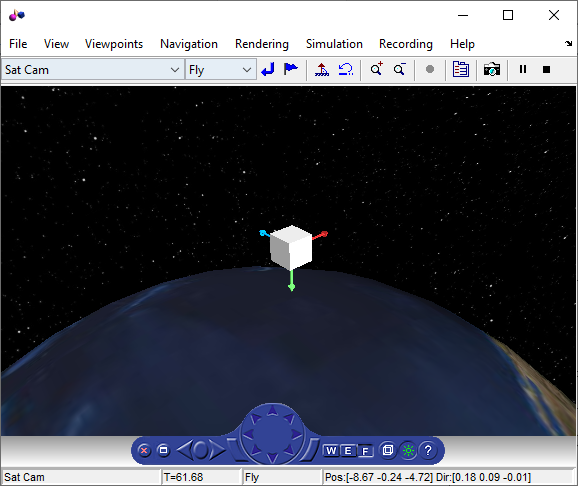
\includegraphics[width=1\textwidth, height=280px]{2-toolbox/vrml.png}
            \caption{Example of Virtual World satellite visualization}
            \label{fig:vrml}
        \end{figure}
        

    \subsubsection{Systems Tool Kit}
        \ac{stk}, formerly named Satellite Tool Kit, is a platform for analyzing and visualizing variety of ground, sea and space platforms missions. \ac{stk} is a commercial software solution used by most major organizations and companies such as \ac{nasa}, \ac{esa}, \ac{dlr}, Boeing, ICEYE. Features most relevant to the topic of this thesis are the graphical engine allowing for displaying the position and attitude of the satellite, and the set of analytical tools, such as ground station connection time calculator, allowing for fine-tuning of mission details.

        To visualize \ac{scars} simulation results with \ac{stk}, one must generate timestamped ephemeris and attitude files. \ac{scars} can generate such files for the user, with predetermined format according to \ac{stk} documentation\cite{stkephemeris}. Both files contain the preamble specifying parameters such as scenario epoch time, central body, coordinate system, distance unit and format of the file. As \ac{scars} relies mostly on \ac{ecef} reference frame, it is also chosen for ephemeris and attitude files. After the preamble, the file contains the lines for each data point. In case of ephemeris file  (\verb|.e| file) the have a format of:

        \begin{Verbatim}[fontsize=\small]
<TimeInSeconds> <X> <Y> <Z> <xDot> <yDot> <zDot>
        \end{Verbatim}

        Where the unit of time is seconds and relative to defined scenario epoch and following parameters are \ac{ecef} vectors in $m$, $m/s$ and $m/s^2$ respectively. For the attitude file (\verb|.a| file), the format is:
        
        \begin{Verbatim}[fontsize=\small]
<TimeInSeconds> <q1> <q2> <q3> <q4>
        \end{Verbatim}
        
        Where time is formatted in same manner as in ephemeris file and the following parameters build a quaternion vector, with fourth element being scalar component.

        Example \verb|.e| and \verb|.a| files can be found in \autoref{app:efile} and \autoref{app:afile} respectively.

        %https://help.agi.com/stk/11.0.1/Content/stk/importfiles-02.htm#timePosVelAcc

        \begin{figure}[H]
            \centering
            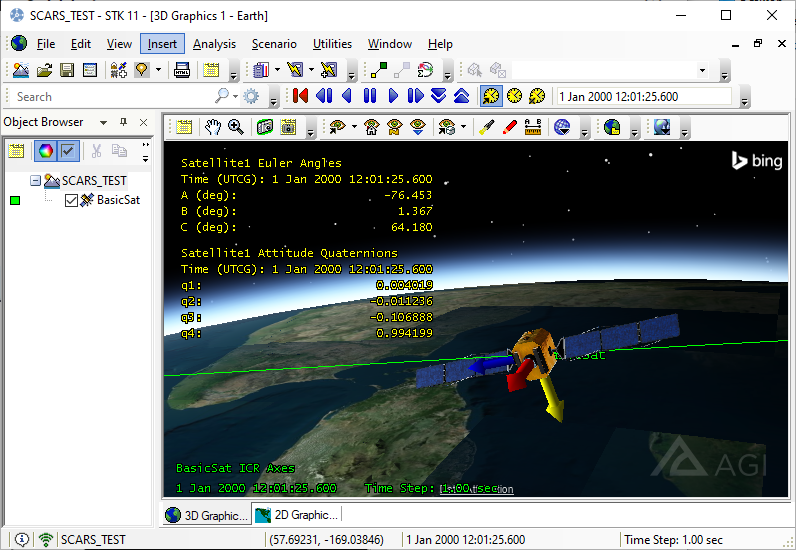
\includegraphics[width=1\textwidth]{2-toolbox/stk_3d.png}
            \caption{Example of STK 3D satellite visualization}
            \label{fig:stk-3d}
        \end{figure}

        \begin{figure}[H]
            \centering
            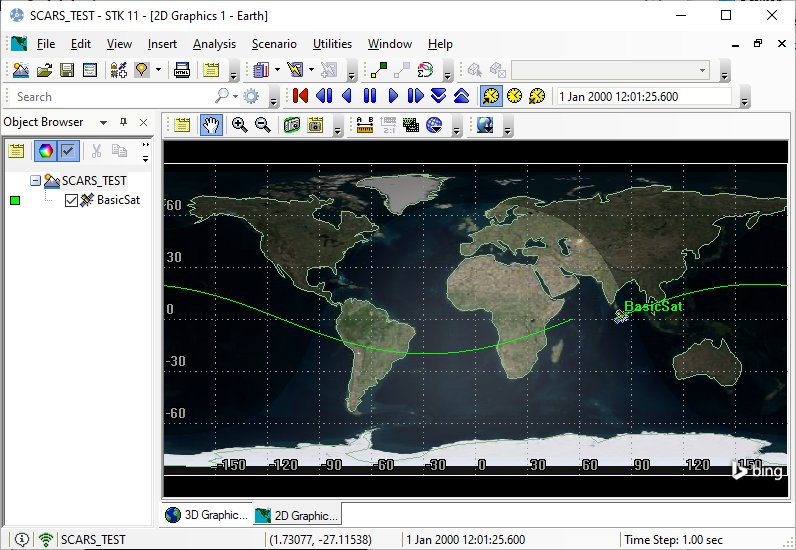
\includegraphics[width=1\textwidth, height=280px]{2-toolbox/stk_groundtrack.png}
            \caption{Example of STK ground track representation}
            \label{fig:stk-ground}
        \end{figure}

        Data produced by a simulation of a simple model, consisting only of \textbf{Environment} and \textbf{Satellite Dynamics} blocks created with SCARS Toolbox was exported into  \verb|.e| and \verb|.a|, from which first lines are shown in mentioned Appendixes. The results were imported into \ac{stk} and can be seen on \autoref{fig:stk-3d} and \autoref{fig:stk-ground}.


    \subsubsection{Kerbal Space Program}\label{sec:ksp}
        Finally, \ac{ksp}, a space flight simulation video game, can be used as a nonconventional method to visualize the results of \ac{scars} Toolbox simulation. In \ac{ksp} the player directs a developing space program originated on fictional Earth-like planet Kerbin. The game provides the tools for the players to design and fly rockets, probes, satellites, spaceplanes, rovers, and other spacecraft from a library of components.\cite{kerbals} The aim of this visualization method was to build a sample satellite in \ac{ksp}, simulate it in \ac{scars} and execute a Hohmann Transfer within a game, using simulation outputs as game inputs.

        The connection between MATLAB and \ac{ksp} is possible because of fanmade \ac{krpc} mod. It creates a API server running alongside the game, with which calls can be made using already written clients in most popular languages, like C++, Python, Lua, Java, etc. Integrating it with MATLAB has proved to be a difficult task, as MATLAB doesn't provide simple means for threading, which means that inputs for the game have to be precalculated to work in real time. Moreover, there is no \ac{krpc} library written directly for MATLAB, therefore a simple Python bridge was written to parse the data taken from the game, compare them with pre-generated \ac{scars} simulation scenario outputs and send them to \ac{ksp} as in-game \ac{aocs} subsystem inputs.

        \begin{figure}[H]
            \centering
            \includegraphics[width=1\textwidth, height=100px]{example-image-b}
            \caption{Example of kRPC Python client code}
            \label{fig:krcp}
        \end{figure}

        \dots\textit{rest description and screenshots of visualization}\dots
\section{Documentation of SCARS}
\subsection{MATLAB Masks and help}
\subsection{Website?}
\section{Example of usage}\label{sec:examples}

\subsection{Setting up spacecraft ADCS architecture in SCARS}

\subsubsection{Basic made up spacecraft}

\subsubsection{PW-Sat2}
    Magnetorquers

    Two modes of control: Detumbling Control Mode; Sun Pointing Mode
    % https://pw-sat.pl/wp-content/uploads/2014/07/PW-Sat2-C-01.00-ADCS-CDR.pdf

    \paragraph*{Deorbitation with drag sail}\hspace{0pt} \\
        One of the main objectives of PW-Sat2 mission was to deploy and test the effectiveness of it's drag sail in deorbitation maneuver. The sail was  $2$x$2m$ square made from aluminized polyester boPET film.\cite{pwsat2dt}
        
        In this example, \ac{scars} toolbox was tested against data points derived from NORAD measurements. The simulation was run in two cases: only with drag sail set up and with drag sail and magnetorquers on to keep sail's plane perpendicular to spacecraft's orbit tangent vector.
         
        \begin{figure}[H]
            \centering
            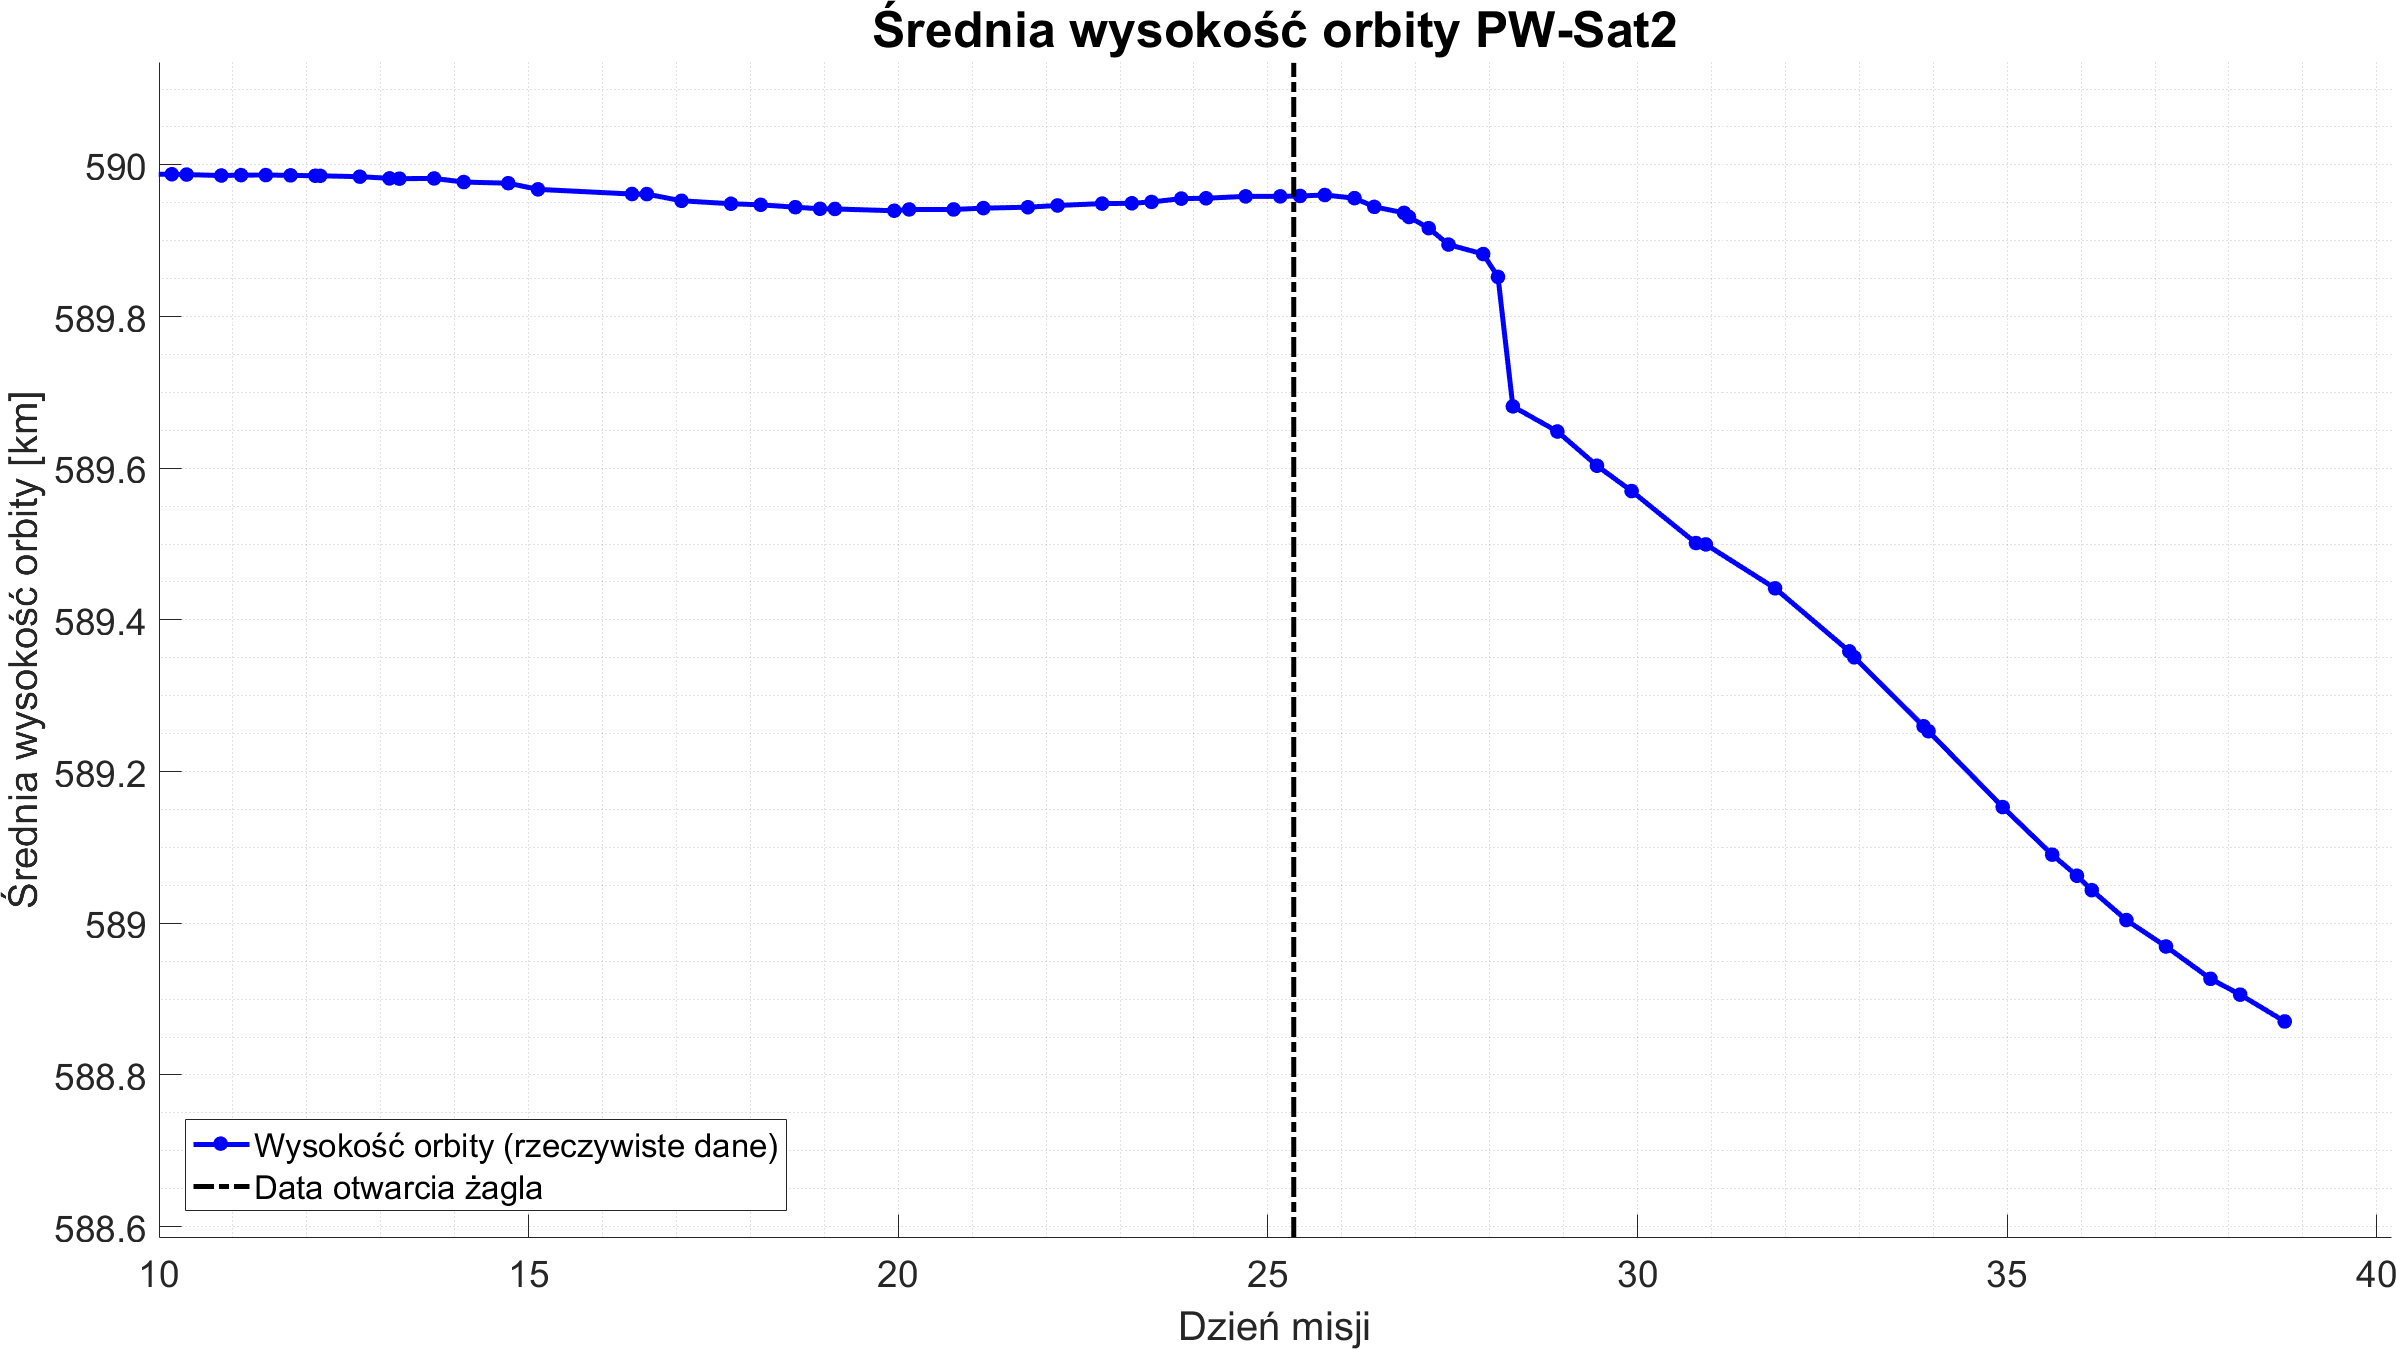
\includegraphics[width=1\textwidth]{4-examples/pw-sat-deorbit.png}
            \caption{Average altitude of PW-Sat2 satellite as taken from NORAD measurements. On X axis there is mission time in days, on Y axis there is average altitude in km.}
            \label{fig:pw-sat-deorbit}
        \end{figure}
         
        \begin{figure}[H]
            \centering
            \includegraphics[width=1\textwidth, height=160px]{example-image-a}
            \caption{Results from \ac{scars} simulation, with only drag sail included}
            \label{fig:scars-deorbit}
        \end{figure}
         
        \begin{figure}[H]
            \centering
            \includegraphics[width=1\textwidth, height=160px]{example-image-b}
            \caption{Results from \ac{scars} simulation, with magnetorquer-driven attitude correction}
            \label{fig:scars-deorbit}
        \end{figure}


    % \subsubsection{PROBA-1}
    % https://directory.eoportal.org/web/eoportal/satellite-missions/p/proba-1#spacecraft


    \subsubsection{Sentinel-2} 
    
    Sentinel-2 is a European polar satellite mission carried out by \ac{esa} as a part of Copernicus Programme. It consists of constellation of twin polar orbit satellites, Sentinel-2A and Sentinel-2B and it's aim is to deliver Earth observation data to broad public, providing wide range of services such as natural emergency management, agricultural monitoring or water classification. \cite{sentinelreference_description}

    As per document describing Sentinel-2 \ac{adcs} subsystem, the satellites operate on a sun-synchronous oribt, with $786km$ mean altitude and $10:30$ local time of descending node. They maintain Earth-oriented attitude in all operational modes. The required pointing performance is moderate, but the main design driver is the need for precise geo-location of the images. \cite{sentinelreference_adcs}

    The actuators on board of Sentinel-2 and simulated with \ac{scars} toolbox for demonstration purposes are decribed in Table \ref{table:sentinel-adcs}.

    % Gyro: https://spaceequipment.airbusdefenceandspace.com/avionics/fiber-optic-gyroscopes/astrix-200/
    % Thrusters: https://www.yumpu.com/en/document/read/10860453/1-n-monopropellant-thruster-astrium-st-eads
    % Magnetometer: http://www.zarmtec.uni-bremen.de/products/magnetometer/
        
    \begin{center}    
        \begin{tabular}{ c l l l l }
            No. & Unit & Type & Supplier & Name \\ \hline
            3 & MAG & 3-axis fluxgate magnetometer & ZARM Technik & FGM-A-75 \\
            2 & GPRS & 2 band GPS receiver & RUAG & - \\
            3 & STR  & Active pixel sensor star tracker & Jena Optronik & Astro APS \\
            4 & IMU & High performance fibre optical gyro & Astrium & ASTRIX 200 \\
            3 & MTQ & $140 Am^2$ magnetic torquer & ZARM Technik & MT140-2\\
            4 & RW & $18 Nms$ reaction wheel & Honeywell & HR12 \\
            8 & THR & $1N$ monopropellant thruster & EADS ST &CHTIN-6
        \end{tabular}
    \end{center}\label{table:sentinel-adcs}

\subsection{Examples of tests possible with SCARS}

\subsubsection{Control system robusntess analisys}

\subsubsection{Long term simulation}

\subsubsection{Contingency scenarios}

\section{Conclusions}\label{sec:conclusions}

    \subsection{Problems encountered}
        It was a mistake to try to build simulation for both fast maneuvers and long term mission planning.

\bibliographystyle{unsrt}
\bibliography{misc/bibliography}
\clearpage

\begingroup
\renewcommand{\arraystretch}{1} %
\setlength{\parskip}{0cm}

\listoffigures

\listoftables
\endgroup
\clearpage

\section*{Appendices}
\addcontentsline{toc}{section}{Appendices}
\appendix
\renewcommand{\thesubsection}{\Alph{subsection}}
\subsection{Example STK Ephemeris File}\label{app:efile}
    \dots\textit{code}\dots

\subsection{Example STK Attitude File}\label{app:afile}
    \dots\textit{code}\dots
\subsection{Model Linearization with Control System Toolbox}\label{app:linearization}
    % \dots\textit{explanation}\dots
    This appendix contains the step-by-step instructions to linearize the chosen SCARS model. In the case of this example, the aim is to acquire linear model of satellite with added actuators, to use it for control system design. The relevant block in this SCARS model are \textbf{Satellite Dynamics} as a core of simulation, one \textbf{Reaction Wheel (1-axis, X/Y/Z)} for each major axis. \autoref{fig:lin_model} presents the whole model used in this example.

    \makeatletter 
    \renewcommand{\thefigure}{C.\@arabic\c@figure}
    \makeatother

    \begin{figure}[H]
        \centering
        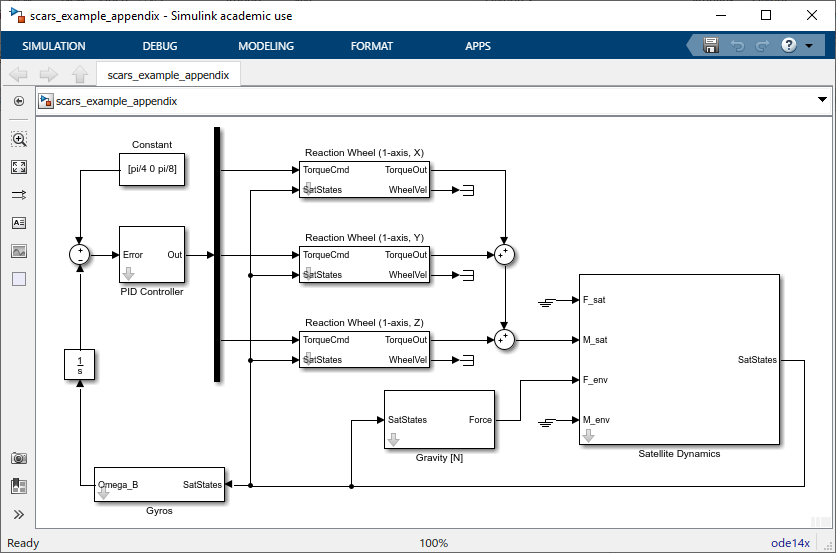
\includegraphics[width=1\textwidth]{appendix/lin_model.png}
        \caption{Satellite model built with SCARS for purposes of linearization presentation}
        \label{fig:lin_model}
    \end{figure}


        
    \subsubsection*{Step 1: Create output signals}

        To linearize the SCARS model one has to determine inputs and outputs which will be represented by the acquired linearized model. While the model inputs are same as the actuators blocks inputs (or \textbf{Demux} outputs), the outputs have to be extracted from \textbf{SatStates} bus. To do that, the user has to add \textbf{Bus Selector} block and choose, in case of this example, \textbf{Euler\_B} signal, as seen on \autoref{fig:lin_selector}. 
        
        It has to be noted that if any controller is set up to provide input signal, like \textbf{PID Controller} in this example, it has to be commented out from the model before linearization.
        % \vfill
        \begin{figure}[H]
            \centering
            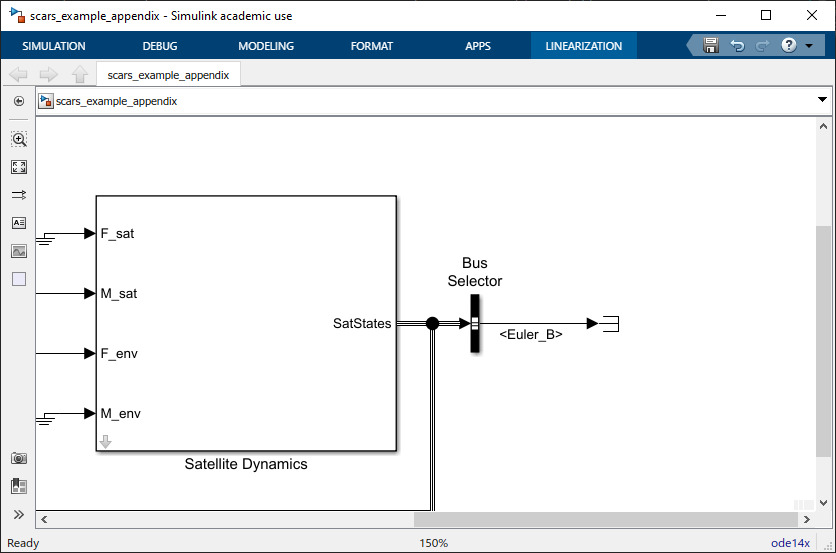
\includegraphics[width=1\textwidth]{appendix/bus_selector.png}
            \caption{Extraction of output signal from bus port}
            \label{fig:lin_selector}
        \end{figure}
        % \vfill

    \subsubsection*{Step 2: Select input and output signals}

        Once all signals are available in the model, it is necessary to properly mark them for Simulink Linear Analysis Tool. To do that, the user has to open \textit{Linearization Manager} from \textit{Apps} tab in Simulink model editor. Then, a signal has to be chosen and in \textit{Linearization} tab a correct type of signal has to be applied. In case of input it has to be \textit{Open-loop Input}, as seen on \autoref{fig:lin_io} \subref{sub:lin_input}, and in case of output it has to be \textit{Open-loop Output}, as seen on \autoref{fig:lin_io} \subref{sub:lin_output}. Small arrow icons over the signal route show that the I/O ports are properly set up.

        \begin{figure}[H]
            \centering
            \subfloat[Open loop input setup]{{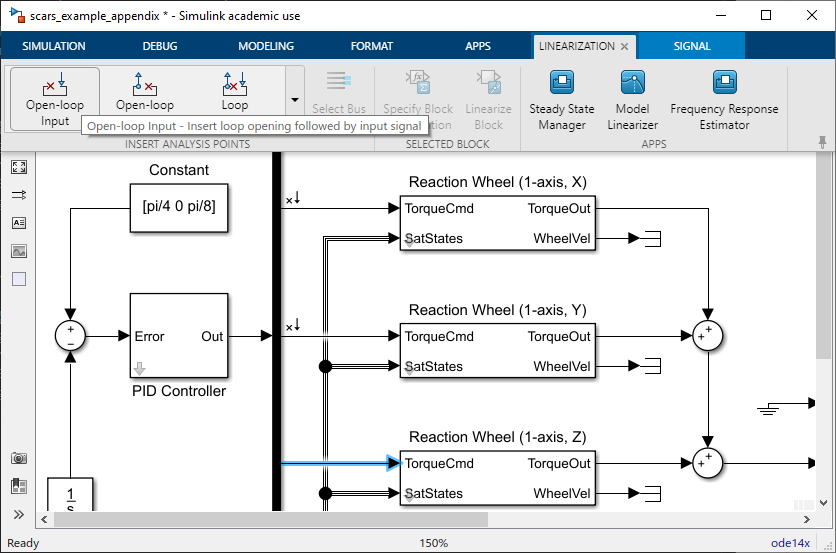
\includegraphics[width=0.97\textwidth]{appendix/input.png}\label{sub:lin_input} }}%
            % \qquad
            \\
            \subfloat[Open loop output setup]{{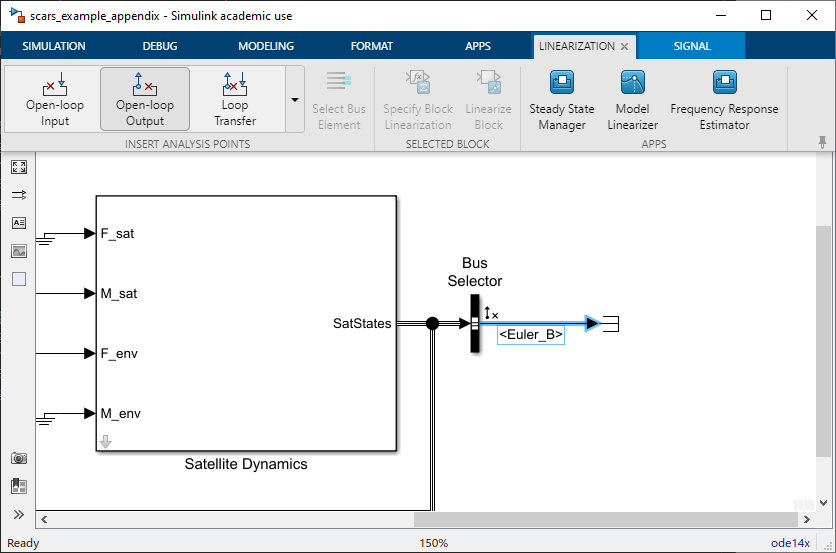
\includegraphics[width=0.97\textwidth]{appendix/output.png}\label{sub:lin_output} }}%
            \caption{Step 2: Open loop I/O setup}%
            \label{fig:lin_io}%
        \end{figure}

        

    \subsubsection*{Step 3: Trim the model}
        After setting up the model I/O signals, the user can open \textit{Linear Analysis Tool} by choosing \textit{Model Linearizer} from either \textit{Apps} or \textit{Linearization} tabs. Once loaded, the initial conditions have to be set up for the linearization process. To do that, the user can trim the model by choosing \textit{Trim Model...} from \textit{Model Initial Condition} in \textit{Setup} section of \textit{Linear Analysis} tab.
         
        For this example, the only checkboxes that need to be marked in opened dialog are \textit{Steady State} for all three states of both \verb|Satellite Dynamics/6DOF ECEF| \verb|(Quaternion)/p,q,r| and \verb|Satellite Dynamics/Euler_B|, as can be seen on \autoref{fig:lin_trimming}. After that the user has to click the \textit{Start trimming} button.

        \begin{figure}[H]
            \centering
            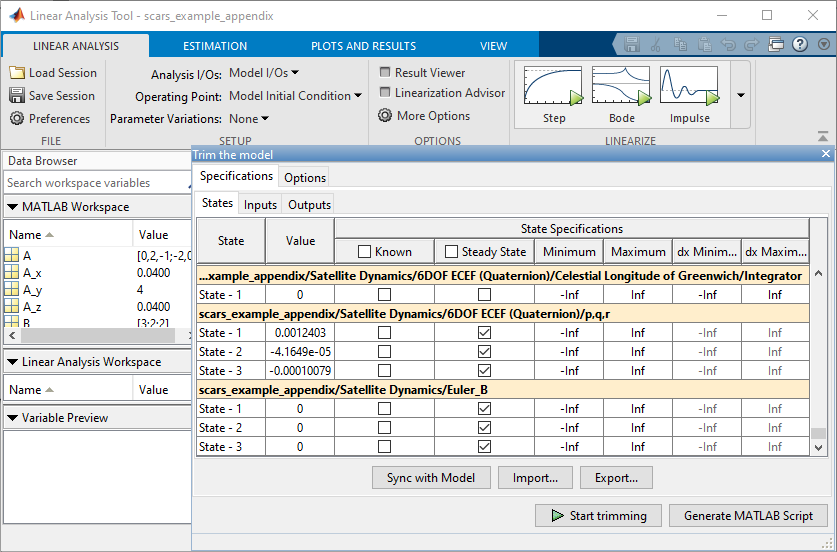
\includegraphics[width=1\textwidth]{appendix/trimming.png}
            \caption{Model trimming}
            \label{fig:lin_trimming}
        \end{figure}

        

    \subsubsection*{Step 4: Linearization of the model}
        Once the model has been trimmed the initial conditions are automatically set. Then, the user can launch linearization process from \textit{Linearize} section of \textit{Linear Analysis} tab, by choosing any plot or option there. This should result in a plot (if chosen) and linearized model available in \textit{Linear Analysis Workspace}, under the name \verb|linsys1| or similar. The user can then move it it \textit{MATLAB Workspace} and use it for various purposes, such as control system design as presented in example in \autoref{sec:control_design}.

        \begin{figure}[H]
            \centering
            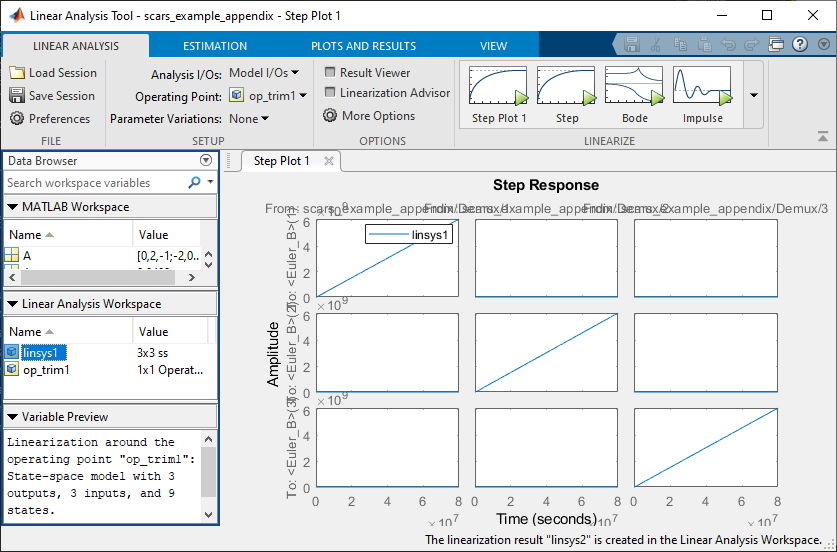
\includegraphics[width=1\textwidth]{appendix/linear.png}
            \caption{Linear Analysis Tool window after successful linearization}
            \label{fig:lin_linear}
        \end{figure}

\end{document}
